%Version 2.1 April 2023
% See section 11 of the User Manual for version history
%
%%%%%%%%%%%%%%%%%%%%%%%%%%%%%%%%%%%%%%%%%%%%%%%%%%%%%%%%%%%%%%%%%%%%%%
%%                                                                 %%
%% Please do not use \input{...} to include other tex files.       %%
%% Submit your LaTeX manuscript as one .tex document.              %%
%%                                                                 %%
%% All additional figures and files should be attached             %%
%% separately and not embedded in the \TeX\ document itself.       %%
%%                                                                 %%
%%%%%%%%%%%%%%%%%%%%%%%%%%%%%%%%%%%%%%%%%%%%%%%%%%%%%%%%%%%%%%%%%%%%%

%%\documentclass[referee,sn-basic]{sn-jnl}% referee option is meant for double line spacing

%%=======================================================%%
%% to print line numbers in the margin use lineno option %%
%%=======================================================%%

%%\documentclass[lineno,sn-basic]{sn-jnl}% Basic Springer Nature Reference Style/Chemistry Reference Style

%%======================================================%%
%% to compile with pdflatex/xelatex use pdflatex option %%
%%======================================================%%

%%\documentclass[pdflatex,sn-basic]{sn-jnl}% Basic Springer Nature Reference Style/Chemistry Reference Style


%%Note: the following reference styles support Namedate and Numbered referencing. By default the style follows the most common style. To switch between the options you can add or remove “Numbered” in the optional parenthesis. 
%%The option is available for: sn-basic.bst, sn-vancouver.bst, sn-chicago.bst, sn-mathphys.bst. %  
 
%%\documentclass[sn-nature]{sn-jnl}% Style for submissions to Nature Portfolio journals
%%\documentclass[sn-basic]{sn-jnl}% Basic Springer Nature Reference Style/Chemistry Reference Style
\documentclass[sn-mathphys,Numbered]{sn-jnl}% Math and Physical Sciences Reference Style
%%\documentclass[sn-aps]{sn-jnl}% American Physical Society (APS) Reference Style
%%\documentclass[sn-vancouver,Numbered]{sn-jnl}% Vancouver Reference Style
%%\documentclass[sn-apa]{sn-jnl}% APA Reference Style 
%%\documentclass[sn-chicago]{sn-jnl}% Chicago-based Humanities Reference Style
%%\documentclass[default]{sn-jnl}% Default
%%\documentclass[default,iicol]{sn-jnl}% Default with double column layout

%%%% Standard Packages
%%<additional latex packages if required can be included here>

\usepackage{graphicx}%
\usepackage{multirow}%
\usepackage{amsmath,amssymb,amsfonts}%
\usepackage{amsthm}%
\usepackage{mathrsfs}%
\usepackage[title]{appendix}%
\usepackage{xcolor}%
\usepackage{textcomp}%
\usepackage{manyfoot}%
\usepackage{booktabs}%
\usepackage{algorithm}%
\usepackage{algorithmicx}%
\usepackage{algpseudocode}%
\usepackage{listings}%
\usepackage{subcaption}
\usepackage{tikz}
\usetikzlibrary{decorations.pathmorphing}



%%%%

%%%%%=============================================================================%%%%
%%%%  Remarks: This template is provided to aid authors with the preparation
%%%%  of original research articles intended for submission to journals published 
%%%%  by Springer Nature. The guidance has been prepared in partnership with 
%%%%  production teams to conform to Springer Nature technical requirements. 
%%%%  Editorial and presentation requirements differ among journal portfolios and 
%%%%  research disciplines. You may find sections in this template are irrelevant 
%%%%  to your work and are empowered to omit any such section if allowed by the 
%%%%  journal you intend to submit to. The submission guidelines and policies 
%%%%  of the journal take precedence. A detailed User Manual is available in the 
%%%%  template package for technical guidance.
%%%%%=============================================================================%%%%

%\jyear{2021}%

%% as per the requirement new theorem styles can be included as shown below
\theoremstyle{thmstyleone}%
\newtheorem{theorem}{Theorem}%  meant for continuous numbers
%%\newtheorem{theorem}{Theorem}[section]% meant for sectionwise numbers
%% optional argument [theorem] produces theorem numbering sequence instead of independent numbers for Proposition
\newtheorem{proposition}[theorem]{Proposition}% 
%%\newtheorem{proposition}{Proposition}% to get separate numbers for theorem and proposition etc.

\theoremstyle{thmstyletwo}%
\newtheorem{example}{Example}%
\newtheorem{remark}{Remark}%

\theoremstyle{thmstylethree}%
\newtheorem{definition}{Definition}%

\raggedbottom
%%\unnumbered% uncomment this for unnumbered level heads

\begin{document}

\title[Article Title]{Lifshitz motivated black holes in two-dimensional dilaton gravity}

%%=============================================================%%
%% Prefix	-> \pfx{Dr}
%% GivenName	-> \fnm{Joergen W.}
%% Particle	-> \spfx{van der} -> surname prefix
%% FamilyName	-> \sur{Ploeg}
%% Suffix	-> \sfx{IV}
%% NatureName	-> \tanm{Poet Laureate} -> Title after name
%% Degrees	-> \dgr{MSc, PhD}
%% \author*[1,2]{\pfx{Dr} \fnm{Joergen W.} \spfx{van der} \sur{Ploeg} \sfx{IV} \tanm{Poet Laureate} 
%%                 \dgr{MSc, PhD}}\email{iauthor@gmail.com}
%%=============================================================%%

\author[1]{\fnm{Uriel} \sur{Noriega-Cornelio}}\email{uriel.noriegacor1@alumno.buap.mx}

\author[2]{\fnm{Alfredo} \sur{Herrera-Aguilar}}\email{aherrera@ifuap.buap.mx}

\author[1]{\fnm{Cupatitzio} \sur{Ramírez-Romero}}\email{cramirez@fcfm.buap.mx}

\affil[1]{\orgdiv{Facultad de Ciencias Físico Matemáticas}, \orgname{Benemérita Universidad Autónoma de Puebla}, \orgaddress{\street{Ciudad Universitaria}, \city{Puebla}, \postcode{CP 72570}, \state{Puebla}, \country{México}}}

\affil[2]{\orgdiv{Instituto de Física}, \orgname{Benemérita Universidad Autónoma de Puebla}, \orgaddress{\street{Edificio IF-1, Ciudad Universitaria}, \city{Puebla}, \postcode{CP 72570}, \state{Puebla}, \country{México}}}

%%==================================%%
%% sample for unstructured abstract %%
%%==================================%%

\abstract{In this paper, we present four novel analytic Lifshitz motivated black hole solutions in a two-dimensional dilaton gravity theory, which contains two scalar fields non-minimally coupled to gravity. Our solutions I and II contain two arbitrary integration constants in the blackening factor $f(r)$, with which we can impose a novel extremality condition, in contrast with previously known black hole field configurations. Solution I coincides with a previously reported AdS black hole when one of the integration constants vanishes in $f(r)$, the critical exponent is set to unity, and we have only one non-trivial scalar field. Solutions III and IV correspond to extreme black hole configurations with an asymptotically finite constant dilaton field. For all of our solutions, we show that $AdS_2$ spacetime arises as the geometry outside the extremal black hole configurations, not only in the near horizon region, regardless of the critical exponent value $z$. In order to elucidate their black hole nature, we explore the causal structure of solutions I and II with the aid of suitable Kruskal-like coordinates and Penrose diagrams. By employing the Hamilton-Jacobi method, we construct a boundary counter-term that renders a renormalized action with a vanishing variation. We use this finite action for the partition function in the semi-classical approximation. We establish a consistent Thermodynamics, verified by the first law, across all the black hole solutions presented, including the extremal cases.}
%%================================%%
%% Sample for structured abstract %%
%%================================%%

% \abstract{\textbf{Purpose:} The abstract serves both as a general introduction to the topic and as a brief, non-technical summary of the main results and their implications. The abstract must not include subheadings (unless expressly permitted in the journal's Instructions to Authors), equations or citations. As a guide the abstract should not exceed 200 words. Most journals do not set a hard limit however authors are advised to check the author instructions for the journal they are submitting to.
% 
% \textbf{Methods:} The abstract serves both as a general introduction to the topic and as a brief, non-technical summary of the main results and their implications. The abstract must not include subheadings (unless expressly permitted in the journal's Instructions to Authors), equations or citations. As a guide the abstract should not exceed 200 words. Most journals do not set a hard limit however authors are advised to check the author instructions for the journal they are submitting to.
% 
% \textbf{Results:} The abstract serves both as a general introduction to the topic and as a brief, non-technical summary of the main results and their implications. The abstract must not include subheadings (unless expressly permitted in the journal's Instructions to Authors), equations or citations. As a guide the abstract should not exceed 200 words. Most journals do not set a hard limit however authors are advised to check the author instructions for the journal they are submitting to.
% 
% \textbf{Conclusion:} The abstract serves both as a general introduction to the topic and as a brief, non-technical summary of the main results and their implications. The abstract must not include subheadings (unless expressly permitted in the journal's Instructions to Authors), equations or citations. As a guide the abstract should not exceed 200 words. Most journals do not set a hard limit however authors are advised to check the author instructions for the journal they are submitting to.}

\keywords{Black Holes, Dilaton-Gravity, 2D Gravity, Lifshitz Black Holes, Extremal Black Holes.}

%%\pacs[JEL Classification]{D8, H51}

%%\pacs[MSC Classification]{35A01, 65L10, 65L12, 65L20, 65L70}

\maketitle

\section{Introduction}
\label{sec:intro}
    
         The gauge/gravity correspondence \cite{Maldacena}, based on the relationship between a gravitational background and a quantum field theory living at the boundary, has shown to be a valuable tool for studying strongly coupled field theories. This approach has been applied to the research in  condensed matter theories \cite{Hartnoll1,Hartnoll2,Hartnoll3,Horowitz,Herreras}, particularly those that  exhibit Lifshitz scale invariance 
        \begin{align} \label{Lifshitz symmetry}
            &t\rightarrow t'=\lambda^z t, &
            &x_i\rightarrow x_i'=\lambda x_i,
        \end{align}
        where the parameter $z$, determining the anisotropy of scaling between time and space, is known as the dynamical critical exponent, $\lambda$ is an arbitrary constant and $i$ labels the spatial dimensions. 
        
        The gravity dual for non-relativistic field theories, with the Lifshitz symmetry (\ref{Lifshitz symmetry}) and $z\neq 1$, is given by the metric \cite{Kachru}  
        %
        \begin{equation} \label{Lifshitz metric}
        ds=l^2 \left(-r^{2z}\;dt^{2}+\frac{dr^2}{r^2}+r^{2} dx_i dx^i\right),    
        \end{equation}
        %
          here $l$ stands for the Lifshitz radius. This metric is invariant under translations, spatial rotations and the anisotropic scale transformation (\ref{Lifshitz symmetry}), provided that the extra coordinate $r$ transforms as $r\rightarrow r'=\lambda^{-1} r$. A detailed review of Lifshitz spacetime and its application to holography can be found in \cite{Taylor1,Taylor2} and references therein.
    
        In the gauge/gravity duality, the nongravitational system in thermal equilibrium at temperature $T$  is in direct correspondence with a black hole with the Hawking temperature $T$. A Lifshitz black hole in $D+1$ dimensions
        is described by 
        %
        \begin{equation} \label{}
        ds=l^2 \left(-r^{2z}\;f(r)\;dt^{2}+\frac{dr^2}{r^2\;f(r)}+r^{2} \;dx_i dx^i\right),
        \end{equation}
        %
        where the function $f(r)$, known as the blackening factor, must asymptotically approach unity in order to recover the Lifshitz background (\ref{Lifshitz metric}) at infinity. 
        Several analytic Lifshitz black hole solutions have been found in the literature within the framework of different field theories \cite{Bertoldi,Tarrio,Ayon1,Azeyanagi,Ayon2,Balasubramanian,Korovin,Shu,Pedraza,Herrera Higuita Mendez,Herreras Higuita}.

%----- Motivation of 2d----- 
% ----motivation with SYK    
    In this paper we present four families of new Lifshitz motivated black hole analytical solutions within the framework of a two-dimensional dilaton gravity theory, with two scalar fields non-minimally coupled to gravity and a metric given by
%
\begin{equation} \label{ansatz}
    ds=l^2 \left(-r^{2z}\;f(r)\;dt^{2}+\frac{dr^2}{r^2\;f(r)}\right).
\end{equation}
Two-dimensional black holes have been studied extensively in the literature, as they serve as models for testing ideas about the physics and Thermodynamics of black holes, with the intention to give insight into quantum gravity in higher dimensions. The Lifshitz motivated black hole solutions with two scalar fields presented here pursue the aim of contributing in this direction by incorporating the anisotropic critical exponent into play 
and serving as a toy model that can be straightforwardly generalized to higher dimensions.

Moreover, dilaton gravity models with one or multiple scalar fields have been used to study holographically non-conformal field theories with an underlying generalized conformal structure \cite{Marika syk}. These theories are scale invariant, provided that their couplings also scale. The structure of these models is captured by Ward identities, relating the stress-energy tensor and scalar operators, which imply restrictions to the correlation functions of the scalar operators. The Sachdev-Ye-Kitaev (SYK) theory has an associated generalized conformal structure, studied holographically by two-dimensional dilaton gravity models with one or multiple scalar fields. It has been shown that the Ward identities governing this structure are obtained by means of the dual two-dimensional dilaton gravity theories. Black hole solutions in these models present thermodynamic properties characterized by a parameter related to the dimension of an AdS black hole parent —the 2D model is obtained by a dimensional reduction of this AdS theory. Interestingly, the black hole solution I that we present here develops the same thermodynamic pattern, with the parameter being the dynamical critical exponent $z$. Besides, our black hole configuration possesses an additional term with an independent integration constant in the blackening factor (see below).

% --------AdS-----------------
As exemplified above, two-dimensional dilaton gravity models are frequently found in the literature as a result of dimensional reductions of systems in higher dimensions. The most known example is the extremal Reissner-Nordstr\"{o}m (RN) black hole solution of four-dimensional Einstein-Maxwell gravity, see for instance \cite{Stanford}. In this example, near $AdS_2$ ($N AdS_2$) spacetime arises as the near-horizon geometry of the near-extremal RN black hole. For all of our two-dimensional black hole solutions presented, we encounter the extremality condition with a relation  between 
the constants of integration in the metric. Interestingly, in this extremal scenario, we found that the $AdS_2$ spacetime emerges as the geometry outside the event horizon (not only near the horizon) of our extremal Lifshitz motivated black holes, regardless of the value of the dynamical critical exponent $z$. This fact is essential to our solutions in the extremal regime, given that $AdS_2$ is a maximally symmetric spacetime invariant under the $SO(2, 1)$ group. This invariance is relevant in the AdS/CFT duality because it corresponds to the conformal invariance of the theory living on the $AdS_2$ boundary.

%-----  Kruskal methods-------
    
    Thus, with the aim of studying the global spacetime structure of some of our black hole solutions, we employ an Eddington-Finkelstein type transformation of coordinates to show the causal structure of spacetime through the behavior of the light cones. Then, we construct a set of Kruskal patches, and corresponding diagrams, adequate to explore the regions containing the outer and inner horizons for our solutions I and II. We depict interesting properties of these spacetimes making use of the appropriate Penrose diagram.
    
%--- Thermodynamics methods---
    
    In particular, it is possible to deduce the thermodynamic quantities for black holes in two dimensions using the Euclidean path integral approximation for the partition function \cite{Gibbons}
%
\begin{equation} \label{aproximation partition function}
\mathcal{Z} \sim \exp \left(-\frac{1}{\hbar} I_E\right),
\end{equation}
%
where $I_E$ represents the Euclidean action evaluated in the classical solutions of  the field equations and $\hbar$ is the Planck constant. In order to use the saddle point approximation in (\ref{aproximation partition function}), it is necessary to have an action that is finite on-shell and whose variation $\delta I$ vanishes. In general, these conditions are not necessarily met by an action. As in higher dimensions, the on-shell action might diverge. This issue is commonly solved by the method of background subtraction \cite{Gibbons}, \cite{Liebl}, which has been applied, for example, to study the Thermodynamics of the Witten black hole \cite{Perry, McGuigan,Nappi}. For our black hole solution I, presented below,  both the on-shell action and $\delta I$ diverge. Following the techniques developed in \cite{Davis} and generalized in \cite{Grumiller}, we apply the method of Hamilton-Jacobi \cite{Martelli} to remove the aforementioned divergences. This method is based on constructing a boundary counter-term that renders a renormalized action $\Gamma$ with suitable properties 
to be used in the approximation (\ref{aproximation partition function}). Once we have the improved action $\Gamma$ at hand, 
we compute the Thermodynamics of all the black hole configurations in the canonical ensemble using the standard approach and show that our field configurations accomplish the first law, even in the extremal cases.
    
    
    In the remainder of this paper, in section \ref{sec2}, we present the four families of Lifshitz motivated black hole solutions in two dimensions, considering two scalar fields, that solve the field equations derived from the corresponding scalar-tensor theory action. In section \ref{sec3}, we extend the spacetime of solutions I and II, transforming first to Eddington-Finkelstein coordinates, and then to Kruskal coordinates designed to go through the outer and inner horizons; finally we present the Penrose diagram for these spacetimes. In section \ref{sec4}, we develop a consistent Thermodynamics for all the black hole configurations presented in this work. In order to do it, first we deduce the Hawking temperature by demanding regularity of the Euclidean spacetime with periodic time. We then show in detail how to construct the counter-term  for the scalar-tensor or dilaton gravity theory in two dimensions considered here, obtaining in this manner a renormalized action. This enables us to employ the approximation (\ref{aproximation partition function}) to deduce consistent thermodynamic properties by means of the first law fulfillment. We compute the total energy $M$ for the black hole solutions employing the gravitational Hamiltonian. Finally, we conclude in section \ref{sec5}.
   


\section{2-dimensional scalar-tensor theory and Lifshitz motivated black holes} \label{sec2}
We shall start by considering the following action in $D+1$ dimensions 
%
\begin{equation} \label{action}
    S = \int d^{D+1} x \sqrt{-g} \; e^{\sum_{a} \gamma_a \phi_a} \left ( R + \sum_{b,c} \beta_{bc} (\partial^{\mu} \phi_b)(\partial_{\mu} \phi_c) - 2 \Lambda \right ),
\end{equation}
%
where $R$ is the Ricci scalar, $g$ is the determinant of the metric, $\Lambda$ is the cosmological constant, $\phi_a$ are the scalar fields, $\gamma_a$ are arbitrary real constant numbers, $\beta_{bc}$ stands for a square symmetric matrix whose elements are arbitrary real constant numbers, and $a$, $b$, $c$ $= 1$, $2$,...,$n$, where $n$ is the number of scalar fields. The action (\ref{action}) has been employed in  \cite{Marika syk} to realize, holographically,
the generalized conformal structure \cite{Jevicki,Jevicki2,Jevicki3} of theories involving multiple scalar field operators, such as the SYK theory \cite{Sachdev,Kitaev}.

The equations of motion following from this action are 
%
\begin{equation}\label{ec einstein}
    \begin{split}
        &R_{\mu \nu} + \sum_{a,b} \beta_{ab} \;\partial_{\mu} \phi_a \;\partial_{\nu} \phi_b - \frac{1}{2} g_{\mu \nu} \left (R + \sum_{a,b} \beta_{ab} \; \partial^{\rho} \phi_a \; \partial_{\rho} \phi_b - 2\Lambda \right )- \sum_a \gamma_a \nabla_{\mu} \partial_{\nu} \phi_a -\\ 
        &\sum_{a,b} \gamma_a \gamma_b \;\partial_{\mu} \phi_a \;\partial_{\nu} \phi_b +g_{\mu \nu} \left ( \sum_{a,b} \gamma_a \gamma_b \;\partial^{\rho}\phi_a \;\partial_{\rho} \phi_b + \sum_a \gamma_a \nabla^2 \phi_a \right )= 0,
    \end{split}
\end{equation}
%
and the scalar field equations
%
\begin{equation}
            \gamma_a \left[ R+\sum_{b,c} \beta_{bc} \;\partial^\sigma \phi_b \;\partial_\sigma \phi_c- 2\Lambda \right]
        =2 \sum_{c} \beta_{ac} \left( \nabla^{2} \phi_c + \nabla^{\mu} \phi_c \sum_{d}\gamma_d \;\partial_\mu \phi_d \right),
\end{equation}        
here a slight difference is noted in comparison to \cite{Marika syk} where the factor $2$ is missing at the right-hand side of this equation.

Under the ansatz (\ref{ansatz}) and considering a static configuration of two scalar fields we arrive at the following Einstein field equations

\textbf{rr:}
%
\begin{equation}\label{eq rr}
    \begin{aligned}
    &\beta _{11} \phi _1'(r){}^2+\beta _{22} \phi _2'(r){}^2+ 2 \beta _{12}  \phi _1'(r)\phi _2'(r)+\gamma _1  \left(\frac{2 z}{r}+\frac{f'(r)}{f(r)}\right)\phi _1'(r)+\\
    &\gamma _2 \left(\frac{2 z}{r}+\frac{f'(r)}{f(r)}\right)\phi _2'(r)+\frac{2 l^2 \Lambda}{r^2 f(r)}=0,
    \end{aligned}
\end{equation}
%

\textbf{tt:}
\begin{equation}\label{eq tt}
    \begin{aligned}
       &\gamma_1 \phi_1''(r) + \gamma_2 \phi_2''(r) +\left( \gamma_{1}^2 - \frac{\beta_{11}}{2} \right) \phi_{1}'(r)^2 + \left( \gamma_{2}^2 - \frac{\beta_{22}}{2} \right) \phi_{2}'(r)^2+\\
       &\left(2\gamma_1 \gamma_2 - \beta_{12}\right) \phi_1 '(r) \phi_2 '(r) + \left(\frac{1}{r}+\frac{f'(r)}{2 f(r)}\right)\left(\gamma_1\phi _1'(r)+\gamma_2 \phi _2'(r)\right)+\\
       &\frac{l^2 \Lambda}{r^2 f(r)}=0,
    \end{aligned}
\end{equation}
%
and the scalar field equations
%
\begin{equation}\label{scalar eq1}
    \begin{split}
        &2 \beta _{11} \phi _1''(r)+ 2 \beta _{12} \phi _2''(r)+\beta _{11} \gamma _1 \phi _1'(r){}^2+\left(2 \beta _{12} \gamma _2-\beta _{22} \gamma _1\right) \phi _2'(r){}^2+\\
        &2 \beta _{11} \gamma _2 \phi _1'(r)\phi _2'(r) + 2\left(\frac{z+1}{r}+\frac{f'(r)}{f(r)}\right)\left( \beta _{11}\phi _1'(r)+ \beta _{12} \phi _2'(r)\right)+\\
        &\frac{\gamma _1 }{r^2 f(r)}\left[ r^{2} f''(r)+(3z+1) r f'(r)+2 z^2f(r)+2 l^2 \Lambda\right]=0,
    \end{split}
\end{equation}
%
\begin{equation}\label{scalar eq2}
    \begin{split}
        &2 \beta _{12} \phi _1''(r)+ 2 \beta _{22}\phi _2''(r)+\left( 2 \beta _{12} \gamma _1-\beta _{11} \gamma _2\right) \phi _1'(r){}^2+\beta _{22} \gamma _2 \phi _2'(r){}^2+\\
        &2 \beta _{22} \gamma _1 \phi _1'(r)\phi _2'(r) + 2 \left(\frac{z+1}{r}+\frac{f'(r)}{f(r)}\right)\left(\beta _{12} \phi _1'(r)+ \beta _{22} \phi _2'(r)\right)+\\
        &\frac{\gamma _2 }{r^2 f(r)}\left[ r^{2} f''(r)+(3z+1) r f'(r)+2 z^2f(r)+2 l^2 \Lambda\right]=0.
    \end{split}
\end{equation}

\subsection{Lifshitz motivated black hole solutions} \label{seccion de soluciones}
In this section we present some analytic black hole solutions for the previous equations of motion. Given that the scalar field solutions $\phi_1$ and $\phi_2$ were obtain keeping the constants $\gamma_1$ and $\gamma_2$ completely arbitrary we consider to rescale the scalar fields so that $\gamma_1=\gamma_2=1$.

\textbf{Solution I.} In this case we consider the relation among the constants $\Lambda=-\frac{z^2}{l^2}$ and $\beta_{11}= \frac{\left(\beta_{12}\right)^2} {\beta_{22}}$. It can be shown that the field equations admit the following Lifshitz motivated black hole solution
\begin{equation} \label{blackhole I}
    ds^2=l^2\left[-\left(1-\frac{c_1}{r^z}+\frac{c_2}{r^{2z}}\right)r^{2z}\;dt^{2}+\frac{dr^2}{ \left(1-\frac{c_1}{r^z}+\frac{c_2}{r^{2z}}\right) \;r^2} \right],
\end{equation}
where $c_1$, $c_2$ are arbitrary real constants.

The scalar fields that support this metric are
%
\begin{align}
    &\phi_1(r)= c_3+  log\left[ \left( r^z - \frac{c_1}{2} \right)^{\sigma_1}\right], &
    &\phi_2(r)= c_4 + log\left[ \left( r^z - \frac{c_1}{2}\right)^{\sigma_2}\right],
\end{align}
where $c_3$, $c_4$ are arbitrary real constants, $\sigma_1=\frac{\beta_{22}}{\beta_{22} -\beta_{12}}$ and $\sigma_2=-\frac{\beta_{12}}{\beta_{22} -\beta_{12}}$ (see Fig. \ref{fig:sol1}).

The outer $r_+$ and inner $r_-$ horizons for this solution are located at
%
\begin{equation} \label{r+-1}
   r_{\pm}= \left(\pm\sqrt{\frac{c_1^2}{4}-c_2}+\frac{c_1}{2} \right)^{\frac{1}{z}}.
\end{equation}

In order to preserve the signature of the metric, that is $f(r)>0$, and for the scalar fields to be well-behaved for $r> r_+> 0$, one of the following two conditions is required
%
\begin{align} \label{caso1i}
    & c_1 > 0,  & \frac{c_{1}^2}{4} &\geq c_2,  & r &> \left(\sqrt{\frac{c_1^2}{4}-c_2}+\frac{c_1}{2}\right)^{\frac{1}{z}},\\
    &c_1 \leq 0,  &  c_2 &\leq 0,  & r &> \left(\sqrt{\frac{c_1^2}{4}-c_2}+\frac{c_1}{2}\right)^{\frac{1}{z}}. \label{caso1ii}
\end{align}

An important remark is that this solution reproduces, as a particular case when $z=1$ and $c_1=0$, the two-dimensional AdS black hole configuration in the group of the $a$-$b$ family of solutions in \cite{Grumiller,Katanaev}, for $b=1$. 

\begin{figure} 
%
\begin{subfigure}{0.5\textwidth}
\includegraphics[width=0.9\linewidth, height=5.5cm]{images/sol1fi1_v2.pdf}
\caption{$\phi_1(r)=-2\;log\left(r^{z}-2\right)$}
\label{fig:subim1}
\end{subfigure}
%
\begin{subfigure}{0.5\textwidth}
\includegraphics[width=0.9\linewidth, height=5.5cm]{images/sol1fi2_v2.pdf}
\caption{$\phi_2(r)=3\;log\left(r^{z}-2\right)$}
\label{fig:subim2}
%
\end{subfigure}

\caption{Solution I. Behavior of the scalar fields for some values of the critical exponent. For these examples we fix $c_3=c_4=0$, $\beta_{22}=2$,  $\beta_{12}=3$, $c_1=4$, $c_2=3$. The dashed vertical lines represent the event horizon $r_+=3^{\frac{1}{z}}$ for each case.}
\label{fig:sol1}
\end{figure}

\textbf{Solution II.} Provided that $\Lambda=0$,  $\beta_{11}=2\beta_{12}-\beta_{22}$, the equations admit the same Lifshitz motivated black hole solution (\ref{blackhole I}), but for a somewhat different scalar field configuration
%
\begin{align}
    &\phi_1(r)= c_3+  log\left[ \left(r^{2z}-c_1 r^z+c_2\right)^{\sigma_1}\right], &
    &\phi_2(r)= c_4 + log\left[ \left(r^{2z}-c_1 r^z+c_2\right)^{\sigma_2}\right],
\end{align}
where $c_3$, $c_4$ are arbitrary real constants, $\sigma_1=\frac{1}{2\left(\beta_{22} -\beta_{12}\right)}$,  $\sigma_2=-\frac{1}{2\left(\beta_{22} -\beta_{12}\right)}$ (see Fig. \ref{fig:sol2}).
The horizons $r_{\pm}$ for this solution have the same expression (\ref{r+-1}).

Again, in order to preserve the signature of the metric and for the scalar fields to be well-defined for $r>r_+>0$, one of the conditions (\ref{caso1i}) and (\ref{caso1ii}) needs to be fulfilled.
%
\begin{figure}[]

\begin{subfigure}{0.5\textwidth}
\includegraphics[width=0.9\linewidth, height=5.5cm]{images/sol2fi1_v2.pdf} 
\caption{$\phi_1(r)=-\frac{1}{2}log\left(r^{2z}-4r^z+3\right)$}
\label{fig:subim1}
\end{subfigure}
\begin{subfigure}{0.5\textwidth}
\includegraphics[width=0.9\linewidth, height=5.5cm]{images/sol2fi2v_2.pdf}
\caption{$\phi_2(r)=\frac{1}{2}log\left(r^{2z}-4r^z+3\right)$}
\label{fig:subim2}
\end{subfigure}

\caption{Solution II. Examples of curves representing the scalar fields for some particular values of $z$, with $c_3=c_4=0$, $\beta_{22}=2$,  $\beta_{12}=3$, $c_1=4$ and $c_2=3$. For each case, the event horizon is located at $r_+=3^{\frac{1}{z}}$, where the scalar fields have a singular behaviour.}
\label{fig:sol2}
\end{figure}

\textbf{Solution III.}
In this solution we consider $\Lambda= 0$, $\beta_{11} = 2$ and $\beta_{22}= 2\left(\beta_{12} - 1 \right)$. Given these conditions we find the following black hole solution
%
\begin{equation} \label{blackhole III}
    ds^2=l^2\left[-\left(1-\frac{c_1}{2r^z}\right)^2 r^{2z}\;dt^{2}+\frac{dr^2}{ \left(1-\frac{c_1}{2r^z}\right)^2 \;r^2} \right],
\end{equation}
%
with the following scalar field configuration
%
\begin{align} \label{scalars solIII}
    &\phi_1(r) = c_3 + log\left[\left(r^z+c_5 \right)^{\sigma_1}\right] - log\left(r^z- \frac{c_1}{2}\right), &
    &\phi_2(r)= c_4 + log\left[\left(r^z+c_5 \right)^{\sigma_2}\right],
\end{align}
where $c_1$, $c_3$, $c_4$ and $c_5$ are arbitrary real constants, $\sigma_1=\frac{ \beta_{12}-1}{ \beta_{12}-2}$,  $\sigma_2=-\frac{ 1 }{ \beta_{12}-2}$ (see Fig. \ref{fig:sol3}).
The event horizon for this solution is located at
%
\begin{equation} \label{rhi}
   r_H= \left(\frac{c_1}{2} \right)^{\frac{1}{z}}.
\end{equation}

In order to have $f(r)>0$ and the scalar fields to be well-behaved for $r> r_H> 0$, we require that $ c_1>0$, $ \frac{c_1}{2} \geq -c_5$ and $r > \left(\frac{c_1}{2}\right)^{\frac{1}{z}}$.

\begin{figure}[]

\begin{subfigure}{0.5\textwidth}
\includegraphics[width=0.9\linewidth, height=5.5cm]{images/sol3fi1_v2.pdf} 
\caption{$\phi_1(r)=2\;log\left(r^z+3\right)-log\left(r^z-2\right)$}
\label{fig:subim3}
\end{subfigure}
\begin{subfigure}{0.5\textwidth}
\includegraphics[width=0.9\linewidth, height=5.5cm]{images/sol3fi2_v2.pdf}
\caption{$\phi_2(r)=- \;log\left(r^z+3\right)$}
\label{fig:subim4}
\end{subfigure}

\caption{Solution III. Scalar field graphics with $z$ specified and with the following parameter values: $c_3=c_4=0$, $\beta_{22}=1$, $\beta_{12}=3$, $c_1=4$ and $c_5=3$. We observe the regular behaviour of the scalar field $\phi_2(x)$  at the horizon $r_H=2^{\frac{1}{z}}$.}
\label{fig:sol3}
\end{figure}

\textbf{Solution IV.}
In this solution we consider $\Lambda= 0$, $\beta_{11} = \frac{2\left(\beta_{12} -\left(1+\kappa \right)\right)}{1 -\kappa}$ and $\beta_{22}=-\frac{2\left(\beta_{12} \kappa - \left(1+\kappa\right) \right)}{1-\kappa}$, where $\kappa$ is an arbitrary proportionality constant between the scalar fields. Under these conditions we find the same black hole solution given by the metric (\ref{blackhole III}) supported by the following scalar fields
\begin{align}
    &\phi_1(r) = c_3 + log\left[\left(r^z - \frac{c_1}{2} \right)^{\sigma_1}\right], & &\phi_2(r) = c_4 + log\left[\left(r^z - \frac{c_1}{2} \right)^{\sigma_2}\right],
\end{align}
where $c_1$, $c_3$, $c_4$ are arbitrary real constants, $\sigma_1=- \frac{\kappa}{\kappa +1}$,  $\sigma_2=- \frac{1}{\kappa + 1}$. %(see Fig. \ref{fig:sol4}). 
These scalar fields behave similarly to those presented in solution II, since they are singular at the horizon. 

In this solution the black hole event horizon is located at the same expression (\ref{rhi}).
In order to have $f(r)>0$ and well-behaved scalar fields for $r> r_H> 0$, we require $c_1 > 0$ and $r > \left(\frac{c_1}{2}\right)^{\frac{1}{z}}$.

We would like to note here that, the black holes presented in solutions III and IV correspond to extreme configurations, in the sense that the event horizon is the union of an outer and an inner horizon, as a result of the relation between the constants of integration
%
\begin{equation}\label{extrem relation}
    c_2=\frac{c_1^2}{4}.
\end{equation}
%
To clarify this point, we study the spacetime structure of solutions I and II in section \ref{sec3}. 

{\bf Dilaton field.} At this point, it is helpful to define the dilaton field $X(r)$ as the exponential function in the action (\ref{action})
\begin{equation}
   X(r)= e^{\sum_a \phi_a}, 
\end{equation}
here $a=1,2$. As we will corroborate in the following sections, this quantity is essential in two-dimensional dilaton gravity models; for instance, it is associated with a conserved charge, defining in this way the corresponding dilatonic potential and determining the thermodynamical properties of the black holes. In addition, the value of the dilaton field at the horizon is encountered to define the entropy of the non-extremal black holes, giving the dilaton a relevant physical significance. 

Furthermore, even though the scalar fields in the extremal solutions III and IV have an asymptotically singular behavior, as exemplified in Fig. \ref{fig:sol3}, the dilaton fields $X(r)$, in both cases, have a constant and finite behavior at infinity, see Fig \ref{img:dilaton fields}. This property is significant (and unusual in dilatonic models) mainly because it leads to a finite on-shell action that we employ in the semiclassical approximation of the partition function without the necessity of a counterterm action, as we will see below.
%
\begin{figure}[]

\begin{subfigure}{0.5\textwidth}
\includegraphics[width=0.9\linewidth, height=5.5cm]{images/X3.pdf} 
\caption{$X(r)=\frac{r^z+3}{r^z-2}$}
\label{Xa}
\end{subfigure}
\begin{subfigure}{0.5\textwidth}
\includegraphics[width=0.9\linewidth, height=5.5cm]{images/X4.pdf}
\caption{$X(r)=\frac{1}{r^z-2}$}
\label{Xb}
\end{subfigure}

\caption{Graphical representation of some examples of the dilaton fields $X(r)= e^{ \phi_1+\phi_2}$ in the extremal solutions III and IV, in Figure (a) and Figure (b), respectively. We employ the following particular values: $c_3=c_4=0$, $\beta_{22}=1$, $\beta_{12}=3$, $c_1=4$, $c_5=3$ and $\kappa=3$. We observe the asymptotically finite and constant value of the dilaton fields $X(r)$ and their singular behaviour at the horizon $r_H=2^{\frac{1}{z}}$, represented here with the dashed vertical lines.}
\label{img:dilaton fields}
\end{figure}


\textbf{Constant curvature.} Finally, we want to highlight that for all solutions presented above, the curvature scalar derived from the ansatz (\ref{ansatz}) 
%
\begin{equation}
    R=g^{\mu \nu} R_{\mu \nu}= -\frac{r^2 f''(r)+ (1+3z)r f'(r)+2z^2 f(r)}{l^2},
\end{equation}
%
 results in a constant and negative quantity 
\begin{equation} \label{curvature}
    R= -\frac{2z^2}{l^2},
\end{equation}
 upon substitution of the metric function $f(r)$. This expression reveals the constant and negative definite character of our spacetime and, for the non-extremal cases, the generalization of AdS ($z=1$) to arbitrary values of the critical exponent (for the case of the extreme black holes see below).

\subsection{AdS$_2$ geometry}

As commented above, the $AdS_2$ geometry emerges as the near-horizon limit of, for instance, the $4D$ extremal  or near-extremal Reissner-Nordstr\"{o}m (RN) black hole; for a pair of nice reviews see \cite{Sarosi,Trunin}. In this example it is usually  shown that, with an appropriate change of variables, the product of $AdS_2$ space and a two-dimensional sphere $S_2$, with radius equal to the dilaton, is obtained near the event horizon. That suitable change of coordinates makes use of a small parameter that sizes the separation from the horizon; eventually this parameter is set to zero as a part of the near-horizon limit.

As stated in the last section, if the relation (\ref{extrem relation}) is met in our two-dimensional solutions, the black holes become extremal. In this scenario we can implement the following change of coordinates 
%
\begin{equation} \label{our change of coord}
    \begin{aligned}
    &r=\left[\frac{c_1}{2}\left(1+\Tilde{r}\right) \right]^{\frac{1}{z}} & &\text{and} & &t=\frac{2}{c_1 z}\; \Tilde{t},
    \end{aligned}
\end{equation}
%
where there is not a near-horizon parameter and the $\Tilde{r}$ coordinate has its origin at the horizon $r_H=\left(\frac{c_1}{2}\right)^{\frac{1}{z}}$.  

Employing the change of coordinates (\ref{our change of coord}) in the metric describing the extreme black hole solutions (\ref{blackhole III}), the resulting geometry description is given by the metric of the two-dimensional anti-de Sitter spacetime $AdS_2$
%
\begin{equation} \label{AdS2 metric}
    ds^2=\frac{l^2}{z^2} \left(-\Tilde{r}^2\;d\Tilde{t}^2+\frac{d\Tilde{r}^2}{\Tilde{r}^2}\right),
\end{equation}
here we observe that the $AdS_2$ radius $L$ is given by the ratio of the Lifshitz radius $l$ and the dynamical critical exponent $z$. Furthermore, if we compute the scalar of curvature employing the metric (\ref{AdS2 metric}) we obtain the constant and negative result
%
\begin{equation}
    R= -\frac{2}{L^2}= - \frac{2 z^2}{l^2},
\end{equation}
the same as (\ref{curvature}), as expected.

It is important to note that, the fact that there is no need to use a parameter that impose the near-horizon validity of the change of coordinates, tells us that we have an $AdS_2$ spacetime in all the region $r_H<r$. Moreover, we also point out that, despite the constant curvature of our solutions, the global causal structure, that we study in detail in the following section, reveals their black hole nature; see for instance \cite{Lemos} for another example of this kind. 

\section{Black hole global causal structure} \label{sec3}

Employing the coordinates ($t$,$r$), the components of the metric have singularities at the outer and inner horizons. Therefore, in order to extend the spacetime trough this surfaces, we need to construct suitable coordinate patches.

In the case of solutions I and II, for radial null curves, the coordinates $t$ and $r$ are related in the following way 
%
\begin{equation} \label{t from r}
    t=\pm  \frac{1}{z \sqrt{c_1^{2}-4 c_{2}}}\;\log \left|\frac{\sqrt{c_{1}^{2}-4 c_{2}}+c_{1}-2 r^{z}}{\sqrt{c_{1}^{2}-4 c_{2}}-c_{1}+2 r^{z}}\right|+\text{constant},
\end{equation}
%
where the upper/lower sign refers to null curves in the direction of increasing/decreasing $r$ (outgoing/ingoing light rays). 
From relation (\ref{t from r}) we define the coordinate 
%
\begin{equation} \label{r star}
    r^*= \frac{1}{z \sqrt{c_1^{2}-4 c_{2}}}\;\log \left|\frac{\sqrt{c_{1}^{2}-4 c_{2}}+c_{1}-2 r^{z}}{\sqrt{c_{1}^{2}-4 c_{2}}-c_{1}+2 r^{z}}\right|,    
\end{equation}
%
such that $ t=\pm r^* + \text{constant}$.

Now we introduce the null coordinates  
\begin{equation} \label{u and v}
u=t-r^* \quad   \text{and}\quad v=t+r^*,
\end{equation}
  which are properly adapted to the description of null geodesics. It is easy to verify that ingoing null geodesics are described by $v=\text{constant}$ while the outgoing ones obey $u=\text{constant}$. We can use the original coordinate $r$ and replace $t$ with the coordinate $v$ or $u$. For example, if we choose the $(v,r)$ coordinate system, known as ingoing Eddington-Finkelstein coordinates, the metric takes the form
  %
\begin{equation}
        ds^{2}=-r^{2z}\left(1-\frac{c_{1}}{r^{z}}+\frac{c_{2}}{r^{2z}}\right)dv^2+2r^{z-1}dvdr.
\end{equation}
%
We can verify that radial null curves satisfy the following conditions:
%
\begin{equation}
        \frac{dv}{dr}=\left\{ \begin{array}{c l} 0 & \text{ingoing} \\\frac{2}{r^{z+1}\left(1-\frac{c_{1}}{r^{z}}+\frac{c_{2}}{r^{2z}}\right)} & \text{outgoing,} \end{array}\right.
\end{equation}
from which we see that the light cones remain well-behaved at $r_+$ and $r_-$. Furthermore, given that the function $f(r)=1-\frac{c_{1}}{r^{z}}+\frac{c_{2}}{r^{2z}}<0$ for $r_-<r<r_+$ all future directed paths of null or timelike particles are in the direction of decreasing r. This is not the case for the region $0<r<r_-$ where $f(r)>0$, consequently, the future directed paths are not necessarily pointing inwards. Below we study these and other properties of the causal structure of solutions I and II by means of Kruskal coordinates.


\subsection{Kruskal extension}
From definitions (\ref{r star}) and (\ref{u and v}), we see that the surface $r=r_+$ is found to be at $u=\infty$ or $v=-\infty$, so it is a good choice to construct the following null Kruskal coordinates
%
\begin{align} \label{coord Kruskal}
&U_{+}=\mp e^{-\kappa_{+} u}, \quad \quad V_{+}=e^{\kappa_{+} v},
\end{align}
%
where the upper sign in $U_+$ is used for $r>r_+$ and the lower sign for $r_-<r<r_+$; the quantity
%
\begin{equation} \label{surface grav}
\kappa_{+} \equiv \frac{r_{+}^{1+z}}{2} f^{\prime}\left(r_{+}\right)= \frac{z}{2} \sqrt{c_1^2-4c_2}, 
\end{equation}
%
is known as surface gravity\footnote{Given that we are dealing with static spacetimes, the event horizon $r_+$ is a Killing horizon where the Killing vector representing time translations  $\xi^\alpha=\left(\partial_t\right)^\alpha$ becomes null. We can associate to this Killing horizon the quantity $\kappa$ given by the relation
\begin{equation}
    \kappa^{2}=-\frac{1}{2}\left(\nabla^{\beta} \xi^{\alpha}\right)\left(\nabla_{\beta} \xi_{\alpha}\right).
\end{equation}
When evaluated at $r_+$, $\kappa$ is known as the surface gravity $\kappa_+ 
$.}. Here the prime denotes derivatives with respect to $r$ and we have made use of relation (\ref{r+-1}).

In order to have a metric with one timelike coordinate and one spacelike we define the following Kruskal coordinates
%
 \begin{align} \label{T y R}
       &T_+=\frac{1}{2}\left(V_+ + U_+\right), &R_+=\frac{1}{2}\left(V_+ - U_+\right),
   \end{align}
%
in terms of which the metric becomes
%
\begin{equation} \label{metrica T y R}
    d s^2 = 
    %\left(\frac{\sqrt{c_{1}^{2}-4 c_{2}}-c_{1}+2 r^{z}}{z\; \sqrt{c_1^2-4c_2}}\right)^2\left(-dT_+^2+dR_+^2\right)=
    \frac{4}{z^2 \left(T_{+}^2-R_{+}^2+1\right)^2} \left(-dT_+^2+dR_+^2\right),
\end{equation}
%
where we used the following identities 
%
\begin{align}\label{T R de r}
    T_+^2-R_+^2&=U_+V_+=
    1- \frac{2\left(2r^z-c_1\right)}{2r^z-c_1+\sqrt{c_{1}^2-4c_2}}.
\end{align}

The form of the metric (\ref{metrica T y R}) tells us that  solutions I and II are conformally equivalent to flat spacetime.

Using equation (\ref{T R de r}) to evaluate the metric (\ref{metrica T y R}) at  $r_+$ for solutions I and II
\begin{equation}
    ds^2= \frac{4}{z^2}\left(-dT_+^2+dR_+^2\right),
\end{equation}
we appreciate the nonsingular nature of the outer horizon.

Some important remarks for this coordinates are
%
\begin{itemize}
    \item From (\ref{metrica T y R}) we see that radial null curves look like they do in two-dimensional flat spacetime, $T_+=\pm R_+ + \text{constant}$. In particular, from (\ref{T R de r}) we see that the outer horizon $r_+$ is described by the straight lines $T_+=\pm R_+$.
    \item   From equation (\ref{T R de r}) we realize that $r=\text{constant}$ curves are described now by hyperbolae $ T_+^2-R_+^2=\text{constant}$. In particular we see that the Lifshitz boundary $r \rightarrow \infty$ is depicted by  $T_+^{2}-R_+^{2}\rightarrow -1$.
    \item The range for these coordinates is $ -\infty<T_+<\infty$, \ \ $R_+^2< T_+^2+1$.
    \item By virtue of equations (\ref{r+-1}) and (\ref{T R de r}) we see that the inner horizon $r_-$ is located at $T_+^2-R_+^2 \rightarrow \infty$, consequently we need a new set of Kruskal coordinates to extend the spacetime in that direction.
\end{itemize}

We can draw the Kruskal diagram in the plane $T_+-R_+$, as shown in Figure \ref{kruskal diagram}, that illustrates the regions outside (I and IV) and inside (II and III) $r_+$ up to an arbitrary cutoff point $r_1>r_-$. We see that for $r_-<r<r_+$ all null and timelike future directed paths are in the direction of decreasing $r$ revealing that the null surface $r_+$ is an event horizon.
%
\begin{figure}
    \centering
    \includegraphics[scale=.4]{images/kruskal_diagram1_v2.pdf}
    \caption{Kruskal diagram in coordinates ($T_+$, $R_+$).}
    \label{kruskal diagram}
\end{figure}
%

As for the outer horizon $r_+$ case, we construct a new set of Kruskal coordinates, $T_-$ and $R_-$, adapted to the inner horizon $r_-$. In this case we define the null coordinates 
%
\begin{align} \label{coord Kruskal -}
&U_{-}=\mp e^{-\kappa_{-} u}, \quad V_{-}=-e^{\kappa_{-} v},
\end{align}
%
where the upper sign in $U_-$ is used for $r>r_-$ and the lower sign refers to $r<r_-$ and $\kappa_{-}=\frac{r_{-}^{1+z}}{2} f^{\prime}\left(r_{-}\right)$. The surface $r_-$ is located at $v\rightarrow \infty$ or $u\rightarrow -\infty$. As in the previous case we define the following Kruskal coordinates
%
 \begin{align} \label{T y R -}
       &T_{-}=\frac{1}{2}\left(V_- + U_-\right), &R_-=\frac{1}{2}\left(V_- - U_-\right),
   \end{align}
%
in terms of which the metric becomes
%
\begin{equation} \label{metrica T y R -}
    d s^2 =
    \frac{4}{z^2 \left(T_{-}^2-R_{-}^2+1\right)^2} \left(-dT_{-}^2+dR_{-}^2\right),
\end{equation}
%
where we used the identities
\begin{align}\label{T R de r -}
    T_{-}^2-R_{-}^2&= U_-V_-=
    1-\frac{2 \left(2r^z-c_1\right)}{2r^z-c_1-\sqrt{c_{1}^2-4c_2}}.
\end{align}

The former equation (\ref{T R de r -}) becomes identically zero when evaluated at the inner horizon $r_-$ (\ref{r+-1}). Using this fact in equation (\ref{metrica T y R -}), we realize that the metric is manifestly regular at $r_-$, i.e. $ds^2= \frac{4}{z^2} \left(-dT_-^2+ dR_-^2\right)$.  

With this knowledge at hand, we draw the Kruskal diagram, as illustrated in Figure \ref{kruskal diagram 2}, for the region $0<r<r_1$ that contains the inner horizon $r=r_-$. 
\begin{figure}
    \centering
    \includegraphics[scale=.4]{images/kruskal_diagram2_v2.pdf}
    \caption{Kruskal diagram for coordinates ($T_-$, $R_-$).}
    \label{kruskal diagram 2}
\end{figure}
A remarkable feature is that, for $r<r_-$, any surface $r=\text{constant}$ is a timelike surface, including the singularity $r=0$. This is due to the re-interpretation of $r$ as a spacelike coordinate because $f>0$ for $r<r_-$. Because of this, the singularity can be avoided, if so decided, by observers moving within the region $0<r<r_-$ of the black hole, since there, the light cone's direction allows for this kind of motion. We illustrate this interesting feature in the following section.

\subsection{Penrose diagram}

In order to illustrate our two-dimensional Lifshitz motivated spacetimes I and II in compact form, we construct their Penrose diagram, showed in Figure \ref{Penrose diagram}. 

We employ the coordinate transformation 
%
\begin{equation} \label{conformal trans}
    \tilde{U}_{\pm}=arctan(U_{\pm})\;\; \text{and} \; 
    \; \tilde{V}_{\pm} = arctan(V_{\pm}),
\end{equation}
% 
over the null Kruskal coordinates (\ref{coord Kruskal}) and (\ref{coord Kruskal -}). The relations (\ref{T y R}), (\ref{T y R -}) and the range of the coordinates $\left(T_+,R_+\right)$, which is the same for $\left(T_-,R_-\right)$, are employed to deduce that the range of the coordinates $\left(U_+,V_+\right)$ and $\left(U_-,V_-\right)$ is given by
%
\begin{equation}
    -\infty < U_{\pm} < \infty \;\; \text{and} \;\; -1 < U_{\pm} V_{\pm}.
\end{equation}
%
Taking into account this last relation and the transformation (\ref{conformal trans}) we easily realize that the $\left(\tilde{U}_+,\tilde{V}_+\right)$ and $\left(\tilde{U}_-,\tilde{V}_-\right)$ coordinate domains are defined by the intersection of
%
\begin{equation}
    -\frac{\pi}{2} < \tilde{U}_{\pm} < \frac{\pi}{2}, \;\;\; -\frac{\pi}{2} < \tilde{V}_{\pm} < \frac{\pi}{2}  \;\;\text{and} 
    \;\; -1 < tan\left(\tilde{V}_{\pm} \right) tan\left(\tilde{U}_{\pm}\right).
\end{equation}
%

From the relations (\ref{T y R}) and (\ref{T y R -}), the metric expressions (\ref{metrica T y R}) and (\ref{metrica T y R -}), and the transformation (\ref{conformal trans}), we find the metric form
%
\begin{equation}
    ds^2= -\frac{4}{z^2} \frac{d \tilde{U}_{\pm} d\tilde{V}_{\pm}}{cos^2\left(\tilde{U}_{\pm}-\tilde{V}_{\pm}\right)}.
\end{equation}
From this equation we observe that the light cones are depicted with lines $\tilde{U}_{\pm}=$constant or $\tilde{V}_{\pm}=$constant. The outer and inner horizons $r_+$ and $r_-$ are described with the same straight lines $\tilde{U}_{\pm} \tilde{V}_{\pm}=0$ as in Kruskal coordinates. The timelike boundary $r\rightarrow \infty$ is now depicted in a finite form by straight lines between the future timelike infinity $i^+$ and the past timelike infinity $i^-$ which, in the same way, are the past and future end points of the surfaces $r=$constant. Similarly, the singularity $r=0$ is illustrated by straight lines in this conformal diagram.

We use the Penrose diagram to illustrate the motion of an observer inside the Lifshitz black holes I and II, as shown in Figure \ref{Penrose diagram}. Once the observer has crossed the outer horizon $r=r_+$, when moving towards the interior of the event horizon, the only possible direction implies  decreasing $r$, in this region the  coordinate $r$ is timelike. After crossing the inner horizon $r=r_-$ the coordinate $r$ becomes spacelike and any direction is possible. If the observer decides to return to the inner horizon he will cross another copy of $r_-$. After that, the only option for the observer is to go towards the outer horizon because now the coordinate $r$ becomes once again timelike. The observer goes out, from another copy of the outer horizon, to a new asymptotically Lifshitz spacetime.

\begin{figure}
\centering
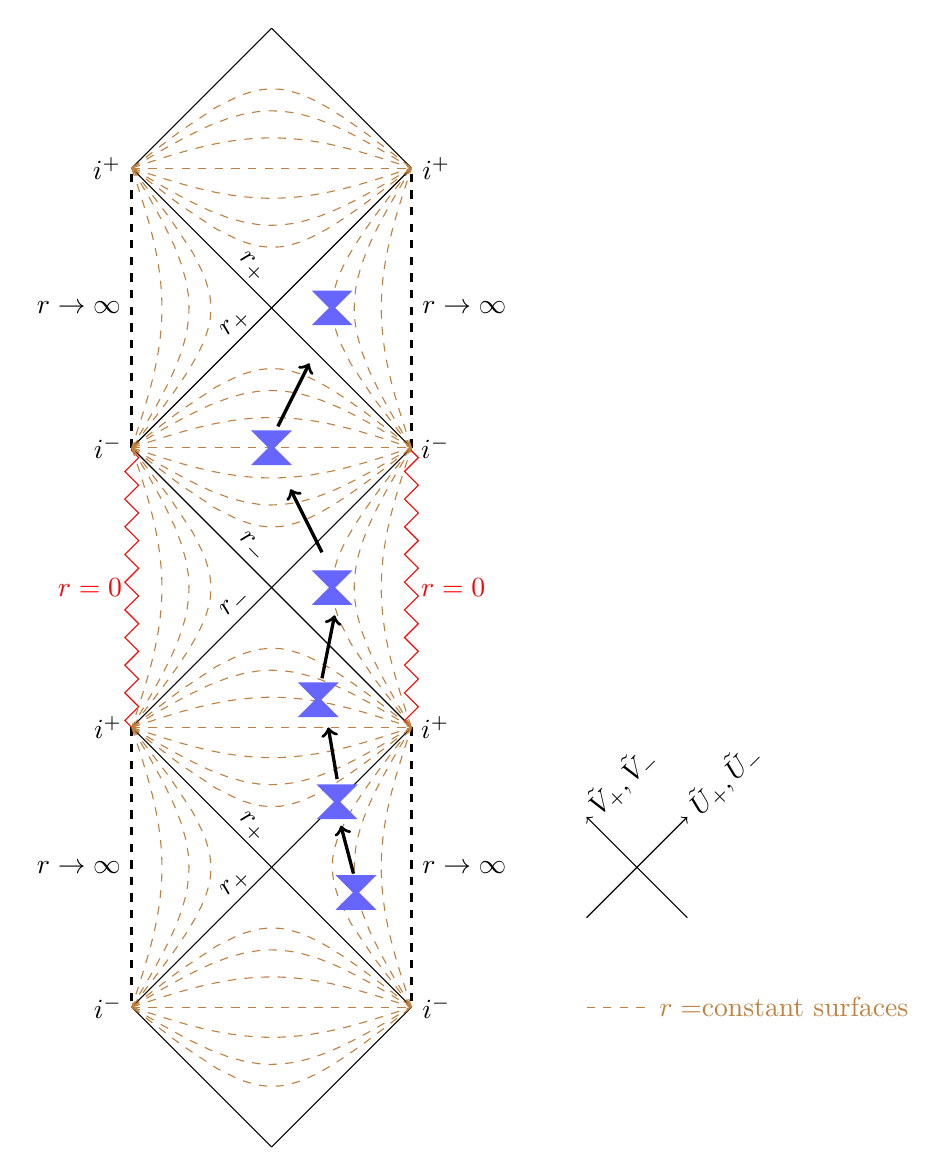
\begin{tikzpicture}[scale=1.6] %\label{Penrose diagram}

% under (part of) horizon r_-
\draw (-1.11,-1.11) -- (0,-2.22);
\draw (1.11,-1.11) -- (0,-2.22);

% lower event horizon r_+ (ORIGIN OF THE COORDINATES)
\draw (-1.11,1.11) node[anchor=east]{$i^+$} --node[pos=0.38,
above=-2.5,
rotate=-45]{$r_+$} 
%node[pos=0.62,above=-2.5,rotate=-45,scale=0.85]{$r_+$}
(1.11,-1.11);
\draw (-1.11,-1.11) node[anchor=east]{$i^-$} --node[pos=0.42,
above=-2.5,
rotate=45]{$r_+$} 
(1.11,1.11) node[anchor=west]{$i^+$};
\draw[dashed,very thick] (-1.11,1.11) --node[anchor=east]{$r \rightarrow \infty$} (-1.11,-1.11);
\draw[dashed,very thick] (1.11,1.11) --node[anchor=west]{$r \rightarrow \infty$} (1.11,-1.11) node[anchor=west]{$i^-$};

% middle horizon r_- 
\draw (-1.11,1.11) --node[pos=0.42,
above=-2.5,
rotate=45]{$r_-$} (1.11,3.33);
\draw (-1.11,3.33) --
node[pos=0.38,above=-2.5,rotate=-45]{$r_-$} (1.11,1.11);

% singularities
\draw [red, decorate, decoration=zigzag](-1.11,1.11) --node[anchor=east]{$r=0$} (-1.11,3.33) ; 
\draw [red, decorate, decoration=zigzag](1.11,1.11) --node[anchor=west]{$r=0$} (1.11,3.33);

% upper event horizon r_+ 
\draw (-1.11,3.33) node[anchor=east]{$i^-$} --node[pos=0.42,
above=-2.5,
rotate=45]{$r_+$}(1.11,5.55);
\draw (-1.11,5.55)--node[pos=0.38,
above=-2.5,
rotate=-45]{$r_+$}(1.11,3.33)node[anchor=west]{$i^-$};
\draw[dashed,very thick] (-1.11,3.33) --node[anchor=east]{$r \rightarrow \infty$} (-1.11,5.55)node[anchor=east]{$i^+$};
\draw[dashed,very thick] (1.11,3.33) --node[anchor=west]{$r \rightarrow \infty$} (1.11,5.55)node[anchor=west]{$i^+$};

% upper (part of) horizon r_-
\draw (-1.11,5.55) -- (0,6.66);
\draw (1.11,5.55) -- (0,6.66);

% Surfaces of constant r

% Lower r_+
%right
\draw[dashed,color=brown,domain=0.001:1.57,rotate=45] plot(\x,{pi/180*atan(-.5/tan(\x r))});
\draw[dashed,color=brown, domain=0.001:1.57,rotate=45] plot(\x,{pi/180*atan(-.25/tan(\x r))});
\draw[dashed,color=brown,domain=0.001:1.57,rotate=45] plot(\x,{pi/180*atan(-.125/tan(\x r))});
\draw[dashed,color=brown](-1.11,-1.11) -- (1.11,-1.11);

%left
\draw[dashed,color=brown,domain=0.001:1.57,rotate=-135] plot(\x,{pi/180*atan(-.5/tan(\x r))});
\draw[dashed,color=brown,domain=0.001:1.57,rotate=-135] plot(\x,{pi/180*atan(-.25/tan(\x r))});
\draw[dashed,color=brown,domain=0.001:1.57,rotate=-135] plot(\x,{pi/180*atan(-.125/tan(\x r))});

%upper
\draw[dashed,color=brown,domain=0.001:1.57,rotate=45] plot(\x,{pi/180*atan(.5/tan(\x r))});
\draw[dashed,color=brown,domain=0.001:1.57,rotate=45] plot(\x,{pi/180*atan(.25/tan(\x r))});
\draw[dashed,color=brown,domain=0.001:1.57,rotate=45] plot(\x,{pi/180*atan(.125/tan(\x r))});
\draw[dashed,color=brown](-1.11,1.11) -- (1.11,1.11);

%lower
\draw[dashed,color=brown,domain=0.001:1.57,rotate=-45] plot(\x,{pi/180*atan(-.125/tan(\x r))});
\draw[dashed,color=brown,domain=0.001:1.57,rotate=-45] plot(\x,{pi/180*atan(-.25/tan(\x r))});
\draw[dashed,color=brown,domain=0.001:1.57,rotate=-45] plot(\x,{pi/180*atan(-.5/tan(\x r))});

\begin{scope}[shift={(0,-2.22)}]
\draw[dashed,color=brown,domain=0.001:1.57,rotate=45] plot(\x,{pi/180*atan(.5/tan(\x r))});
\draw[dashed,color=brown,domain=0.001:1.57,rotate=45] plot(\x,{pi/180*atan(.25/tan(\x r))});
\draw[dashed,color=brown,domain=0.001:1.57,rotate=45] plot(\x,{pi/180*atan(.125/tan(\x r))});
\end{scope}

%Middle r_-

\begin{scope}[shift={(0,2.22)}]
%right
\draw (0,1.11)[dashed,color=brown,domain=0.001:1.57,rotate=45] plot(\x,{pi/180*atan(-.5/tan(\x r))});
\draw[dashed,color=brown, domain=0.001:1.57,rotate=45] plot(\x,{pi/180*atan(-.25/tan(\x r))});
\draw[dashed,color=brown,domain=0.001:1.57,rotate=45] plot(\x,{pi/180*atan(-.125/tan(\x r))});
%\draw[color=brown,domain=0.001:1.57,rotate=45] plot(\x,{pi/180*atan(-.0575/tan(\x r))});

%left
\draw[dashed,color=brown,domain=0.001:1.57,rotate=-135] plot(\x,{pi/180*atan(-.5/tan(\x r))});
\draw[dashed,color=brown,domain=0.001:1.57,rotate=-135] plot(\x,{pi/180*atan(-.25/tan(\x r))});
\draw[dashed,color=brown,domain=0.001:1.57,rotate=-135] plot(\x,{pi/180*atan(-.125/tan(\x r))});

%upper
\draw[dashed,color=brown,domain=0.001:1.57,rotate=45] plot(\x,{pi/180*atan(.5/tan(\x r))});
\draw[dashed,color=brown,domain=0.001:1.57,rotate=45] plot(\x,{pi/180*atan(.25/tan(\x r))});
\draw[dashed,color=brown,domain=0.001:1.57,rotate=45] plot(\x,{pi/180*atan(.125/tan(\x r))});
\draw[dashed,color=brown](-1.11,1.11) -- (1.11,1.11);

%lower
\draw[dashed,color=brown,domain=0.001:1.57,rotate=-45] plot(\x,{pi/180*atan(-.125/tan(\x r))});
\draw[dashed,color=brown,domain=0.001:1.57,rotate=-45] plot(\x,{pi/180*atan(-.25/tan(\x r))});
\draw[dashed,color=brown,domain=0.001:1.57,rotate=-45] plot(\x,{pi/180*atan(-.5/tan(\x r))});
\end{scope}


%Upper r_+
\begin{scope}[shift={(0,4.44)}]
%right
\draw [dashed,color=brown,domain=0.001:1.57,rotate=45] plot(\x,{pi/180*atan(-.5/tan(\x r))});
\draw[dashed,color=brown,domain=0.001:1.57,rotate=45] plot(\x,{pi/180*atan(-.25/tan(\x r))});
\draw[dashed,color=brown,domain=0.001:1.57,rotate=45] plot(\x,{pi/180*atan(-.125/tan(\x r))});
%\draw[color=brown,domain=0.001:1.57,rotate=45] plot(\x,{pi/180*atan(-.0575/tan(\x r))});

%left
\draw[dashed,color=brown,domain=0.001:1.57,rotate=-135] plot(\x,{pi/180*atan(-.5/tan(\x r))});
\draw[dashed,color=brown,domain=0.001:1.57,rotate=-135] plot(\x,{pi/180*atan(-.25/tan(\x r))});
\draw[dashed,color=brown,domain=0.001:1.57,rotate=-135] plot(\x,{pi/180*atan(-.125/tan(\x r))});

%upper
\draw[dashed,color=brown,domain=0.001:1.57,rotate=45] plot(\x,{pi/180*atan(.5/tan(\x r))});
\draw[dashed,color=brown,domain=0.001:1.57,rotate=45] plot(\x,{pi/180*atan(.25/tan(\x r))});
\draw[dashed,color=brown,domain=0.001:1.57,rotate=45] plot(\x,{pi/180*atan(.125/tan(\x r))});
\draw[dashed,color=brown](-1.11,1.11) -- (1.11,1.11);

%lower
\draw[dashed,color=brown,domain=0.001:1.57,rotate=-45] plot(\x,{pi/180*atan(-.125/tan(\x r))});
\draw[dashed,color=brown,domain=0.001:1.57,rotate=-45] plot(\x,{pi/180*atan(-.25/tan(\x r))});
\draw[dashed,color=brown,domain=0.001:1.57,rotate=-45] plot(\x,{pi/180*atan(-.5/tan(\x r))});
\end{scope}

%the uppest part:
\begin{scope}[shift={(0,6.66)}]
\draw[dashed,color=brown,domain=0.001:1.57,rotate=-45] plot(\x,{pi/180*atan(-.125/tan(\x r))});
\draw[dashed,color=brown,domain=0.001:1.57,rotate=-45] plot(\x,{pi/180*atan(-.25/tan(\x r))});
\draw[dashed,color=brown,domain=0.001:1.57,rotate=-45] plot(\x,{pi/180*atan(-.5/tan(\x r))});
\end{scope}

%Light cones

%lower region
%outside r_+
\draw[blue!60, ultra thick,fill=blue!60] (.55,-.32) -- (.79,-.32) -- (.67,-.20) -- cycle;
\draw[blue!60, ultra thick,fill=blue!60] (.55,-.08) -- (.79,-.08) -- (.67,-.20) -- cycle;

\draw[very thick, ->](.65,-.05) -- (.55,.33);

%over r_+
\draw[blue!60,ultra thick,fill=blue!60] (.40,.40) -- (.64,.40) -- (.52,.52) -- cycle;
\draw[blue!60, ultra thick,fill=blue!60] (.40,.64) -- (.64,.64) -- (.52,.52) -- cycle;

\draw[very thick, ->](.52,.7) -- (.45,1.11);


%middle region
%inside r_+

\draw[blue!60, ultra thick,fill=blue!60] (.49,1.45) -- (.25,1.45) -- (.37,1.33) -- cycle;
\draw[blue!60, ultra thick,fill=blue!60] (.37,1.33) -- (.25,1.21) -- (.49,1.21) -- cycle;

\draw[very thick, ->](.40,1.5) -- (.50,2);

%inside r_-
\draw[blue!60, ultra thick,fill=blue!60] (.36,2.34) -- (.60,2.34) -- (.48,2.22) -- cycle;
\draw[blue!60, ultra thick,fill=blue!60] (.36,2.10) -- (.60,2.10) -- (.48,2.22) -- cycle;

\draw[very thick, ->](.4,2.5) -- (.15,3);

%upper region
%outside r_- or inside r_+
\draw[blue!60, ultra thick,fill=blue!60] (-.12,3.45) -- (.12,3.45) -- (0,3.33) -- cycle;
\draw[blue!60, ultra thick,fill=blue!60] (0,3.33) -- (-.12,3.21) -- (.12,3.21) -- cycle;

\draw[very thick, ->](.05,3.5) -- (.3,4);

%outside r_+
\draw[blue!60, ultra thick,fill=blue!60] (.36,4.56) -- (.60,4.56) -- (.48,4.44) -- cycle;
\draw[blue!60, ultra thick,fill=blue!60] (.36,4.32) -- (.60,4.32) -- (.48,4.44) -- cycle;


%Notes
\begin{scope}[shift={(0,-1.11)}]
\draw[<-] (2.5,1.51)node[anchor=west,rotate=45]{$\tilde{V}_+,\tilde{V}_-$} -- (3.3,.71);
\draw[->] (2.5,.71)-- (3.3,1.51)node[anchor=west,rotate=45]{$\tilde{U}_+,\tilde{U}_-$};

\draw[color=brown,dashed](2.5,0) -- (3,0)node[anchor=west]{$r=$constant surfaces};
\end{scope}

\end{tikzpicture}
\caption{Conformal diagram for the asymptotically Lifshitz motivated black holes I and II. The spacetime boundary $r \rightarrow \infty$ is represented by the dashed vertical straight lines and the singularity $r=0$ is depicted by the zigzag vertical ones. Here we illustrate a particular motion through a timelike path.}
\label{Penrose diagram}
\end{figure}

\section{Thermodynamics} \label{sec4}

For higher dimensional black holes, the standard Bekenstein-Hawking relation states that the entropy is always found to be one quarter of the horizon area, in Planck units
%
\begin{equation}
    S=\frac{A_H}{4G}.
\end{equation}
%
It is unclear how to apply this formula for the case at hand, with one spatial dimension. 

 In this section, we tackle this problem by employing the Euclidean treatment of quantum gravity \cite{Gibbons}. In this approach, the partition function $\mathcal{Z}$ is obtained by computing the path integral over the space of all periodic field configurations in Euclidean time. As stated above, the path integral is given by the approximation (\ref{aproximation partition function}) under certain conditions. With this in mind, we construct a renormalized action $\Gamma_{\text{reg}}$ with a regulating boundary $r=r_{\text{reg}}$ and obtain the partition function for the canonical ensemble in this way. Finally, we compute the thermodynamic properties for our black hole configurations. We verify the results by accomplishing the quasi-local form of the first law of Thermodynamics.   

\subsection{Temperature}

In order to deduce the Hawking temperature,  following the approach first presented in \cite{Gibbons}, we consider regularity at the Euclidean horizon. As usual, see for example \cite{Hartnoll4}, we first Taylor expand the metric (\ref{ansatz}) near the outer horizon $r_+$ and obtain
%
 \begin{equation}
        ds^2=l^2\left(-r_{+}^{2z}\left(r-r_+\right)f'(r_+) dt^2+\frac{dr^2}{r_+^2\left(r-r_+\right)f'(r_+)}+...\right).
    \end{equation}
%
Subsequently, we perform the Wick rotation $t \rightarrow -i t=t_E$, and carrying out the change of coordinates
%
\begin{align}\label{rho y eta}
        &r=r_++\frac{r_+^2 f'(r_+)}{4l^2}\rho^2, & &t_E=\frac{2}{f'(r_+)r_+^{z+1}}\eta,
    \end{align}
%
we find the near-horizon Euclidean metric to be
%
 \begin{equation} \label{rindler space}
        ds^2=\rho^2 d\eta^2+d\rho^2+...,
    \end{equation}
%
which we identify as Euclidean space in two dimensions in polar coordinates. In order to avoid a conical singularity at the Euclidean horizon $\rho=0$ it is necessary to take into account the periodicity 
 \begin{align} \label{periodicity}
        &\eta \sim \eta+2\pi, & &\text{which means} & &t_E \sim t_E+\frac{4\pi}{f'(r_+)r_+^{z+1}}.
 \end{align}
 Recalling that if we have a quantum field theory with a Wick rotated periodic time, with period $\beta$, then we have a theory with finite temperature $T=\frac{1}{\beta}$, assuming $\hbar=1$. Therefore we have found that the Hawking temperature of the black hole solutions considered here is
 \begin{equation}\label{hawking temperature}
        T=\frac{f'(r_+)r_+^{z+1}}{4\pi},
    \end{equation}
which, as we can appreciate from  (\ref{surface grav}),  is related to the surface gravity in the following way
%
\begin{equation}\label{hawking temperature with surface g}
        T=\frac{\kappa_+}{2\pi}=\frac{z}{4 \pi}\sqrt{c_1^2-4c_2}.
    \end{equation}
It is easy to see that, the extreme solutions III and IV have zero temperature, because of the relation (\ref{extrem relation}).

As stated above, from equation (\ref{hawking temperature with surface g}) we observe that the dynamical exponent $z$ controls the thermodynamic properties of the black holes presented in this work, analogous to the AdS$_2$ solutions with a parameter related to the dimension of an AdS black hole parent, as reported in \cite{Marika syk}.
Moreover, we see that the temperature (\ref{hawking temperature with surface g}) reproduces as a particular case, when $z=1$ and $c_1=0$, the Hawking temperature for the AdS black hole of the $a$-$b$ family presented in \cite{Grumiller} for $b=1$.

In section \ref{sec 4.2.1}, it will be helpful to relate the Hawking temperature $T$ to a local proper temperature $T_w$ measured at an arbitrary surface $r=r_w>r_+$. Given that the Hawking temperature is established by requiring the periodicity (\ref{periodicity}) in the Euclidean time $t_E$ (or in the coordinate $t$), we can employ the Euclidean relation between $t_E$ (or $t$) and the proper time $\tau_w$ for a static observer placed at $r_w$ 
%
\begin{equation}
    d \tau_w^{2} = g_{tt}(r_w)\; dt_E^{2} =r_{w}^{2z} f(r_w) dt^2,
\end{equation}
to obtain the redshift or Tolman relation\footnote{For asymptotically flat black holes, $g_{tt}\rightarrow 1$ when $r \rightarrow \infty$, therefore, the Hawking temperature $T$ corresponds to the local temperature $T_w$ measured by an observer at infinity.} \cite{Tolman}
%
\begin{equation}\label{tolman factor}
    T_w=\frac{1}{r_{w}^{z} \sqrt{f(r_{w})}} T.
\end{equation}

\subsection{Lifshitz motivated black hole partition function in two dimensions} \label{sec 4.2}

From this section we consider the Euclidean version of the action (\ref{action}) in $1+1$ dimensions
%
\begin{equation}\label{action with gibbons term}
    I= \int _{\mathcal{M}} d^{2} x \sqrt{g} \; X \left ( R + \sum_{b,c} \beta_{bc} (\partial^{\mu} \phi_b)(\partial_{\mu} \phi_c) - 2 \Lambda \right ) +2\int_{\partial \mathcal{M}} d x \sqrt{\gamma}\; X\; K, 
\end{equation}
%
where, as stated above, $X= e^{\sum_a \phi_a}$ stands for the dilaton and $a,b,c=1,2$. We have added the Gibbons-Hawking-York term \cite{Gibbons,York} where $\gamma_{ij}=g_{tt}$ is the induced metric on the boundary\footnote{Because we are dealing with a one-dimensional boundary, the subscripts $i,j$ just keep track of the quantities related to the induced metric.}   $r=$constant, with $r\rightarrow \infty$, and $K$ is the trace of the extrinsic curvature or second fundamental form. 

We compute the thermodynamical properties for the black hole solutions presented in section \ref{seccion de soluciones} employing the partition function $\mathcal{Z}$ given by the path integral weighted by the exponential of the Euclidean action $I$ \cite{Gibbons}
%
\begin{equation}
\mathcal{Z}=\int \mathcal{D} g \mathcal{D} \phi_a \exp \left(-\frac{1}{\hbar} I[g, \phi_a]\right),
\end{equation}
with $\mathcal{D} g$ and $\mathcal{D} \phi_a$ denoting some measure for the metric  and  the scalar fields, respectively.  

We might assume that the dominant contribution for the path integral comes from the solutions to the classical field equations, so that we can approximate 
%
\begin{equation} \label{approximation z}
\mathcal{Z} \sim \exp \left(-\frac{1}{\hbar} I\left[g_{c l}, \phi_{a,c l}\right]\right).
\end{equation}
%
 Nevertheless, in order for the assumption to be valid, it is necessary to have an action that is finite on-shell and whose variation $\delta I$ vanishes for the classical solutions $g_{cl}$ and $\phi_{a,cl}$. 
 
 To evaluate the action (\ref{action with gibbons term}), we shall incorporate an auxiliary regulator $r\leq r_{\text{reg}}$, treating the surface $r=r_{\text{reg}}$ as a finite boundary; we recover the full spacetime by taking the limit $r_{\text{reg}} \rightarrow \infty$. For instance, computing the regulated on-shell action for solution I we arrive at
 %
\begin{equation} \label{I_reg onshell action}
    I_{\text{reg}}=2x_0 z \beta \left[\left(r_{\text{reg}}^z-\frac{c_1}{2}\right)^2+\frac{2\pi}{x_0 z} X_+ T-\left(\frac{c_1^2}{4}-c_2\right)\right],
\end{equation}
%
where $X_+=x_0 \sqrt{\frac{c_1^2}{4}-c_2}$ is the value of the dilaton at the horizon $r_+$, the constant $x_0=e^{c_3+c_4}$ and remember that the period $\beta=\frac{1}{T}$, with $T$ being the Hawking temperature (\ref{hawking temperature with surface g}). Note that the limit $r_{\text{reg}}\to\infty$ in equation (\ref{I_reg onshell action})
diverges for the on-shell action I. Similarly, we further verify that variations of the fields, that preserve the boundary conditions in solution I, lead to 
%
\begin{equation}
    \delta I=\lim_{r \rightarrow \infty} \delta I_{\text{reg}}\rightarrow \infty.
\end{equation}

 
Following the techniques developed in \cite{Davis,Grumiller} we apply the method of Hamilton-Jacobi \cite{Martelli} to remove the divergences. This approach enables us to construct a boundary counter-term  $I_{ct}$ that renders the action finite on-shell and that is extremized  by classical solutions of the field equations. This counter-term action is related to (\ref{action with gibbons term}) in the following way
%
\begin{equation} \label{relation actions}
    I= I_{ct}+ \Gamma,
\end{equation}
where the resulting renormalized action $\Gamma$ is the one we are allowed to employ in the saddle point approximation (\ref{approximation z}). The boundary integral $I_{ct}$ may depend on the fields and only on their tangential derivatives to the boundary in order for the actions $I$ and $\Gamma$ to lead to the same field equations. 

In order to obtain the counter-term, the Hamiltonian derived from the action $I$ is required to satisfy the constraint $\mathcal{H}=0$. For the action (\ref{action with gibbons term}) the associated Hamiltonian density is
%
\begin{equation}\label{Hamiltonian density}
\begin{split} 
 \mathcal{H}&=4\left(\beta_{12}^{2}-\beta_{11} \beta_{22}\right)\left(\pi^{i j} \gamma_{i j}\right)^{2}+\left(\pi_{\phi_{1}}-\pi_{\phi_{2}}\right)^{2}+4\pi^{i j} \gamma_{i j} \left[\left(\beta_{22}-\beta_{12}\right) \pi_{\phi_{1}}+\left(\beta_{11}-\beta_{12}\right) \pi_{\phi_{2}}\right]\\
 & +8\left(\beta_{11}+\beta_{22}-2\beta_{12}\right) X^{2} \Lambda,
\end{split} 
\end{equation}
here the canonical momenta, $\pi^{ij}$ and $\pi_{\phi_a}$, conjugate to the fields  are defined in terms of the change of the fields along the $r$ direction\footnote{For a thorough review of the Hamiltonian formulation for a general dilaton theory see \cite{Dyer}. }.

Varying the action with respect to the fields and evaluating it for a solution of the field equations, momenta  appear as boundary terms 
%
\begin{equation}
    \delta I_{\text{on-shell}}=\int_{\partial \mathcal{M}} d \tau  \sqrt{\gamma}\left[\pi^{ij} \delta \gamma_{ij}+\sum_{a=1}^{2} \pi_{\phi_a} \delta \phi_a\right],
\end{equation}
%
in such a way that we can write them as functional derivatives of the on-shell action with respect to the fields at the boundary
%
\begin{equation}\label{momenta as derivatives}
\pi^{i j}=\frac{1}{\sqrt{\gamma}} \frac{\delta}{\delta \gamma_{i j}}\left(I_{\text{on-shell}}\right), \quad \pi_{\phi_a}=\frac{1}{\sqrt{\gamma}} \frac{\delta}{\delta \phi_a}\left(I_{\text{on-shell}}\right).
\end{equation}

With equation (\ref{Hamiltonian density}) and the result (\ref{momenta as derivatives}), the Hamiltonian constraint $\mathcal{H}=0$ is written as a non-linear functional differential equation for the on-shell action, the Hamilton-Jacobi equation. 

Given that the counter-term action is, in the same way, required to solve the Hamilton-Jacobi equation we must have
%
\begin{equation}\label{Hamilton-Jacobi Ict}
\begin{aligned}
&4\left(\beta_{12}^{2}-\beta_{11} \beta_{22}\right)\left[\gamma_{i j}\; \left(\partial_{\gamma_{i j}}I_{ct}\right)\right]^{2}+\left[\left(\partial_{\phi_{1}}I_{ct}\right)-\left(\partial_ {\phi_{2}}I_{ct}\right)\right]^{2}\\
&+4 \gamma_{i j}\; \left(\partial_{\gamma_{i j}}I_{ct}\right)\left[\left(\beta_{22}-\beta_{12}\right) \left(\partial_{\phi_{1}} I_{ct}\right)+\left(\beta_{11}-\beta_{12}\right) \left(\partial_{\phi_{2}}I_{ct}\right)\right]+8\left(\beta_{11}+\beta_{22}-2 \beta_{12}\right) X^2 \Lambda \gamma_{ij}\\
&=0.
\end{aligned}
\end{equation}
In order to solve the above non-linear differential equation we take advantage of the symmetries that $I_{ct}$ must fulfill.
First, it must be invariant under diffeomorphisms of $\partial \mathcal{M}$, accordingly the boundary integral takes the form 
%
\begin{equation}
    I_{ct}=\int_{\partial \mathcal{M}} d\tau\;\sqrt{\gamma}\; \mathcal{L}_{ct}\left(\phi_1,\phi_2\right),
\end{equation}
%
where the scalar $\mathcal{L}_{ct}$ does not depend on tangential derivatives to the boundary because the scalar fields $\phi_a$ are invariant over time.
Secondly the action (\ref{action with gibbons term}) is invariant under the transformation %\cite{Buscher1}, \cite{Buscher2}
%
\begin{equation} \label{B simetry}
    \begin{aligned}
    g_{tt}&\rightarrow\frac{1}{g_{tt}},\\
    \phi_1 \rightarrow \phi_1+\frac{1}{2} log\left(|g_{tt}|\right), &\quad  \phi_2 \rightarrow \phi_2+\frac{1}{2} log\left(|g_{tt}|\right).
    \end{aligned}
\end{equation}
%
We expect that the resulting action $\Gamma$ respects the symmetries that the action $I$ possesses, therefore $I_{ct}$ must be invariant under (\ref{B simetry}). This is achieved by taking the ansatz:
%
\begin{equation}\label{counter-term}
 I_{ct}=C\int_{\partial\mathcal{M}} d\tau \sqrt{g_{tt}}\; e^{\phi_1+\phi_2},
\end{equation} 
%
where $C$ is an arbitrary constant.

The remaining part is to substitute the above expression for $I_{ct}$ into the Hamilton-Jacobi equation (\ref{Hamilton-Jacobi Ict}), then it is straightforward to determine that
%
\begin{equation} \label{counterterm}
    C= 2 \;\sqrt{-2 \Lambda} \left( \frac{\beta_{11}+\beta_{22}-2\beta_{12}}{\beta_{12}^2-\beta_{11}\beta_{22}+2\left(\beta_{11}+\beta_{22}-2\beta_{12}\right)}\right)^{\frac{1}{2}}.
\end{equation}

According to (\ref{action with gibbons term}), (\ref{relation actions}) and (\ref{counter-term}) the action $\Gamma$ becomes
%
\begin{equation}\label{action2}
\begin{aligned}
        \Gamma &= \int _{\mathcal{M}} d^{2} x \sqrt{g} \; X \left ( R + \sum_{b,c} \beta_{bc} (\partial^{\mu} \phi_b)(\partial_{\mu} \phi_c) - 2 \Lambda \right )
        +2\int_{\partial \mathcal{M}} d x \sqrt{\gamma}\; X\; K \\
        &- C\int_{\partial\mathcal{M}} d\tau \sqrt{\gamma}\; X.
\end{aligned}        
\end{equation}

Returning to the case of solution I, substituting the values for $\Lambda$ and $\beta_{11}$ in (\ref{counterterm}) produces a counter-term with $C=\frac{2z}{l}$. As before, employing the regulatory boundary $r=r_{\text{reg}}$, we compute the regulated on-shell action $\Gamma_{\text{reg}}$ for this case:
%
\begin{equation} \label{reg action}
    \Gamma_{\text{reg}}= 2  x_0 z\beta\left[\left(r_{\text{reg}}^z-\frac{c_1}{2}\right)^2+\frac{2\pi}{x_0 z} X_+ T-\left(\frac{c_1^2}{4}-c_2\right)-r_{\text{reg}}^z \sqrt{f(r_{\text{reg}})} \left(r_{\text{reg}}^z-\frac{c_1}{2}\right)\right].
\end{equation}
%
Removing the regulator by taking the limit
%
\begin{equation} \label{on-shell gamma}
    \lim_{r_{\text{reg}}\to\infty} \Gamma_{\text{reg}}=2  x_0 z \beta \left[\frac{2\pi}{x_0 z} X_+ T-\frac{1}{2}\left(\frac{c_1^2}{4}-c_2\right)\right],
\end{equation}
%
we verify the finite result for the renormalized on-shell action $\Gamma$. Furthermore, we compute that all variations of the fields, preserving the boundary conditions, in solution I lead to 
%
\begin{equation}
    \delta \Gamma=\lim_{r_{\text{reg}} \rightarrow \infty} \delta \Gamma_{\text{reg}}=0.
\end{equation}
%
Considering the result (\ref{on-shell gamma}), we develop the remaining thermodynamic properties for the black hole solution I in the following section.

Equation (\ref{counterterm}) shows that there are no counter-terms for the remaining solutions presented in this work, as $\Lambda=0$ in those cases. However, we find that the on-shell actions for these solutions are appropriate finite actions to be used in the semi-classical approximation. This fact allows us to develop the thermodynamic properties presented below.

\subsection{Canonical ensemble} \label{sec 4.2.1}
In usual Thermodynamics a canonical ensemble is defined by the temperature and a variable determining the size of the system, that is to say, the volume. In \cite{York2} the author designs a system consisting of a spherical cavity, delimited by a cavity wall at radius $r$, enclosing  a black hole at the center. The canonical ensemble of such a system is defined by the local constant temperature $T_w(r)$ and the area of the cavity wall. The size of the system is not specified by spatial volume because the volume of a black hole is not defined at a constant Euclidean time. 

Following the approach consisting in enclosing a black hole in a cavity developed in \cite{Perry, Davis, Grumiller}, here we perform a similar analysis. We give a physical meaning to the surface  $r_{\text{reg}}$ by imagining that it represents the wall of a ``cavity'' $r_w$ that maintains boundary conditions. The local temperature $T_w$ measured at the wall is  given by the Tolman relationship (\ref{tolman factor}). 

In two dimensions we can construct a conserved current $j^{\mu}$ from any regular function $f(\Phi)$ of a scalar field in the following way
%
\begin{equation}
    j^{\mu}=\epsilon^{\mu \nu} \nabla _{\nu}f(\Phi),
\end{equation}
where $\epsilon$ is the Levi-Civita tensor in two dimensions. The associated conserved charge is
\begin{equation}
    D_w=f(\Phi_w)=\int_{\Sigma} dr \sqrt{g_{rr}} \;j_{\mu} n^{\mu},
\end{equation}
where $\Sigma$ is a surface of constant time with unitary normal vector $n^{\mu}$ and a boundary located at $r=r_w$.  Following \cite{Perry} we choose the function $f(\Phi)= X$, with $\Phi \equiv \phi_1+\phi_2$, so that we have the conserved dilaton charge
\begin{equation}\label{dilaton charge}
    D_w=X_w,
\end{equation}
%
where the subscript $w$ indicates us that the charge depends on the location of the wall. Thus equation (\ref{dilaton charge}) gives us the dilaton charge contained within the cavity wall $r_w$. We assign to $X_w$ an analogous role to that of the area of the cavity wall in higher dimensions.

As a result we have designed a cavity delimited by a wall $r_w$ where we keep the temperature $T_w$ and dilaton charge $X_w$ fixed, hence the approximation (\ref{approximation z}) accounts for  the partition function in the canonical ensemble
%
\begin{equation} \label{z with Gamma}
\mathcal{Z}(T_w, X_w)=\text{exp}\left(-\Gamma_w\right),
\end{equation}
%
where we have made $\hbar=1$. 

The corresponding  Helmholtz free energy $F_w$ is given by
%
\begin{equation}\label{free energy 1}
 F_w(T_w, X_w)= T_w\;\text{log}\mathcal{Z}=-T_w\; \Gamma_w(T_w, X_w),
\end{equation}
where again, the subscript reminds us that $F_w$ is the Helmholtz free energy for the system inside the wall $r=r_w$. 

On the other hand, the first law of Thermodynamics corresponding to this canonical ensemble reads
\begin{equation}\label{first law0}
    dE_w=T_w dS_w - \psi_w dX_w,
\end{equation}
where $E_w$ is the internal energy, $S_w$ is the entropy and $\psi_w$ is the chemical potential associated with the dilaton charge, the minus sign is intended to preserve the analogy with pressure in standard Thermodynamics. As usual, see for instance \cite{Reif}, from (\ref{first law0}) and the Legendre transformation 
%
\begin{equation}\label{Legendre trans}
    F_w(T_w,X_w) = E_w(S_w,X_w) - T_w S_w,
\end{equation}
%
we arrive to the equivalent formulation
\begin{equation}
    dF_w=-S_w dT_w-\psi_w dX_w,
\end{equation}
which in turn defines the entropy 
%
\begin{equation}\label{entropy def}
    S_w=-\frac{\partial F_w}{\partial T_w}\bigg\rvert_{X_w},
\end{equation}
and the dilaton chemical potential 
%
\begin{equation}\label{chemical potential0}
    \psi_w=-\frac{\partial F_w}{\partial X_w}\bigg\rvert_{T_w}.
\end{equation}

\subsubsection{Solution I}

Using equations (\ref{tolman factor}), (\ref{reg action}), (\ref{free energy 1}) and the fact that $X_w=x_0\left(r_{w}^z-\frac{c_1}{2}\right)$ for solution I, we calculate $F_w$ and obtain
%
\begin{equation}\label{energía libre}
    F_w=2x_0 z\left(\frac{X_w}{x_0}-\frac{T}{T_w}-\frac{2\pi}{x_0 z}X_+ T_w\right).
\end{equation}
%

Based on (\ref{energía libre}) and (\ref{entropy def}) we compute the entropy of the black hole in this solution as follows
%
\begin{equation}\label{entropía}
    S_w= S=-\frac{\partial F_w}{\partial T_w}\bigg\rvert_{X_w}= 4\pi X_+,
\end{equation}
%
where we have used the relation\footnote{This identity is obtained from equation (\ref{tolman factor}) by rewriting the Tolman factor in terms of $X_w$ and $X_+$.}
%
\begin{equation} \label{T and Tw with X}
\frac{T}{T_w}= \frac{1}{x_0}\sqrt{X_{w}^2-X_{+}^2}.
\end{equation}
%
We observe that the entropy of the black hole does not depend on the location of the wall $r_w$ but on the value $X_+$ of the dilaton at the horizon, just as in higher dimensions it depends on the area of the horizon. A universal form for the expression of the entropy is noted in (\ref{entropía}) when compared to other two-dimensional dilaton gravity models \cite{Grumiller,Davis,Nappi}.

As we deduced in (\ref{chemical potential0}) the chemical potential $\psi_w$ associated to the conserved charge (\ref{dilaton charge}) is 
%
\begin{equation}\label{potencial químico}
    \psi_w=-\frac{\partial F_w}{\partial X_w}\bigg\rvert_{T_w}=2z \left( \frac{T_w}{T}\frac{X_w}{x_0}-1\right),
\end{equation}
where relations (\ref{energía libre}) and (\ref{T and Tw with X}) were used. 

Following Brown and York \cite{Brown} we derive the quasi-local energy $E_w$ from the surface stress-energy-momentum tensor 
%
\begin{equation} \label{Brown stress tensor}
    T^{ij}:=- \frac{2}{\sqrt{\gamma}} \frac{\delta \Gamma}{\delta \gamma_{ij}},
\end{equation}
 by contracting $T^{ij}$ with $\xi_i\;\xi_j$, being $\xi_{i}=\sqrt{g_{tt}}\; \delta^\tau_{i}$ the Killing vector related to time translations. Varying the action (\ref{action2}) we encounter that
\begin{equation}
    T^{ij}=\frac{2x_0z}{\gamma_{ij}}\left(\frac{X_w}{x_0}-\frac{T}{T_w}\right),
\end{equation}
accordingly
%
\begin{equation}\label{internal energy}
\begin{aligned}
    E_w=\xi_i\;\xi_j T^{ij}=2x_0z\left(\frac{X_w}{x_0}-\frac{T}{T_w}\right) \geq 0,
\end{aligned}    
\end{equation}
where the restrictions (\ref{caso1i}) and (\ref{caso1ii}) have been used to assert that $E_w$ is positive or zero.

On the other hand, performing a Legendre transformation on (\ref{Legendre trans}) we obtain that the internal energy $E_w$ should obey 
%
\begin{equation} \label{legendre trans 2}
    E_w(S, X_w)=F_w(T_w, X_w)+ T_w \;S. 
\end{equation}
%
Hence, from equations (\ref{energía libre}) and (\ref{entropía}) we found that
%
\begin{equation} \label{internal energy 2}
    E_w(S,X_w)=2x_0z\left(\frac{X_w}{x_0}-\frac{T}{T_w}\right),
\end{equation}
and we see that the internal energy deduced in this manner is in complete agreement with the result (\ref{internal energy}).

Using the identity (\ref{T and Tw with X}) and the expressions for entropy (\ref{entropía})  and dilaton chemical potential (\ref{potencial químico}) we verify the relation (\ref{first law0}) for the internal energy (\ref{internal energy}) by showing that it obeys the first law of black hole Thermodynamics. 

By taking  the differential of (\ref{internal energy}) we find that  
\begin{equation} \label{first law}
\begin{split}
    dE_w &= 2x_0 z \left[ d\left(\frac{X_w}{x_0}\right)-d\left(\frac{T}{T_w}\right)\right]= 2x_0z \left[ d\left(\frac{X_w}{x_0}\right)-d\left(\frac{1}{x_0}\sqrt{X_{w}^2-X_{+}^2}\right)\right]\\
    &= 2z \left[ \left(1-\frac{X_w}{\sqrt{X_{w}^2-X_{+}^2}}\right)dX_w+\frac{X_+}{\sqrt{X_{w}^2-X_{+}^2}} dX_+\right]\\
    &= 2z \left[ \left(1-\frac{T_w}{T} \frac{X_w}{x_0}\right)dX_w+\frac{T}{\frac{1}{x_0}\sqrt{X_{w}^2-X_{+}^2}} \frac{dS}{2z}\right]\\
    &= -\psi_w\;dX_w+T_w\;dS,
\end{split}    
\end{equation}
where in the third equality we can track back how the divergences in $\psi_w$ and $T_w$ cancel each other at $r_w=r_+$, that is to say, at $X_w=X_+$, verifying that $dE_w$ remains regular for all $r_w \geq r_+$, while in the
fourth equality we used $X_+=\frac{2\pi x_0}{z} T$. Here the subscript $w$ indicates us that equation (\ref{first law}) remains valid no matter where the cavity wall is located along the $r$ coordinate. 

Relation (\ref{first law}) is one of the main results of this section and shows that our black hole configuration possesses a consistent Thermodynamics.

It is important to note that under the extremality condition (\ref{extrem relation}) the entropy (\ref{entropía}) of this black hole vanish, recall that $X_+=x_0 \sqrt{\frac{c_1^2}{4}-c_2}$. Furthermore, it is easy to see that when using relation (\ref{extrem relation}), $\psi_w=E_w=T_w=0$. Hence, the first law is trivially fulfilled in the extremal case.


\textit{Black hole mass.-}
Employing the ADM ($1+1$) decomposition, we compute the Hamiltonian for the Lorentzian  version of the action (\ref{action2}) and arrive at
    \begin{equation}\label{Hamiltonian}
      H=\int_{\Sigma_t} d r\left(N \mathcal{H}+N^r \mathcal{H}_r\right)+\left.\left(N \epsilon +N^r P_{rr}\right)\right|_B,
    \end{equation}
%
 here we foliate the spacetime in space-like hypersurfaces $\Sigma_t$ with boundary $B$, $N$ represents the lapse function and $N^r$ is the shift vector, $\mathcal{H}$ and  $\mathcal{H}_r$ are the Hamiltonian and momentum constraint respectively, $P_{rr}$ denotes the canonical momenta conjugate to the induced metric $g_{rr}$ in $\Sigma_t$. We verify that $\epsilon$ corresponds to the quasi-local energy $E_w$, defined in the second equality of equation (\ref{internal energy}).
 
 Evaluating the Hamiltonian (\ref{Hamiltonian}) with a solution of the field equations we obtain 
%
 \begin{equation}\label{on-shell H}
      H=\left.\left(N \epsilon +N^r P_{rr}\right)\right|_B.
    \end{equation}
% 
As stated in \cite{Horowitz2}, this represents the total energy $M$ for spacetimes whose lapse function does not asymptotically approach unity.

Substituting solution I in equation (\ref{on-shell H}), noting that $P_{rr}=0$ for a static solution and $N=\sqrt{|g_{tt}|}$, we arrive at the total energy of the black hole
%
 \begin{equation}\label{M solI}
      M=N \epsilon \left. \right|_B= \lim_{r_w \rightarrow \infty} N\; E_w = x_0 z\left(\frac{c_1^2}{4}-c_2 \right)= \frac{z}{x_0} X_+^2,
    \end{equation}
%
where we observe that the two constants of integration in the blackening function $f(r)$ are involved in the definition of the black hole mass. As the last equality states, the mass is proportional to the dynamical critical exponent $z$ and to the squared dilaton evaluated at the event horizon.

From (\ref{M solI}) we easily see that the internal energy $E_w$ is asymptotically equal to the mass $M$, red-shifted by the Tolman factor:
 %
 \begin{equation}
     \lim_{r_w \rightarrow \infty} E_w = \lim_{r_w \rightarrow \infty}  \frac{M}{r_w^z \sqrt{f(r_w)}}.
 \end{equation}


\subsubsection{Solution II} \label{section 4.2.2}

In the case of the solution II, we have a constant dilaton. Moreover, the counter-term action  (\ref{counter-term}) obtained by the Hamilton-Jacobi method is identically zero, since $\Lambda=0$, see equation (\ref{counterterm}). However, computing the on-shell action for this solution we find that
%
\begin{equation}
   \Gamma_{\text{reg}}= \Gamma=-\frac{z  c_1}{T},
\end{equation}
%
is a constant value independently of the position of the regulatory boundary $r_{\text{reg}}$. Moreover, evaluating $\delta \Gamma$ for this solution, preserving the boundary conditions, we find that the variation is null. Given these properties, we are allowed to employ the semi-classical approximation (\ref{z with Gamma}) for the partition function, although, in this case the system does not have a dilatonic charge.

Making use of the same definitions as before, we deduce the Helmholtz free energy
%
\begin{equation}
    F_w(T_w,X_w)=-T_w \Gamma=z c_1 \frac{T_w}{T},
\end{equation}
%
which we employ to compute the entropy
%
\begin{equation}
    S_w= S=-\frac{\partial F_w}{\partial T_w}\bigg\rvert_{X_w}= -\frac{z  c_1}{T}.
\end{equation}
%
With these two last results and making use of the Legendre transformation (\ref{legendre trans 2}) we deduce that 
%
\begin{equation}
    E_w=0,
\end{equation}
%
for this black hole solution. This is corroborated by the definition of Brown and York
%
\begin{equation}
    E_w= \xi_i\;\xi_j T^{ij}=-2 \; \xi_i\;\xi_j \pi ^{ij}=0,
\end{equation}
%
where in the second equality we make use of relation (\ref{momenta as derivatives}) and definition (\ref{Brown stress tensor}). In the third equality we employ the result
%
\begin{equation}
    \pi^{ij}=\gamma^{ij} n^{\mu} \nabla_{\mu} X,
\end{equation}
%
for a constant dilaton $X$.

Finally, with the results for $E_w$ and $S$ we easily  realize that the first law 
%
\begin{equation}
    dE_w=T_wdS=0,
\end{equation}
%
is accomplished in a trivial manner.

   \subsubsection{Extremal solutions}


As stated before, solutions III and IV correspond to extreme black hole configurations, meaning that the constants of integration in the metric obey the relation (\ref{extrem relation}), leading us to have a null Hawking temperature T, see (\ref{hawking temperature with surface g}). Because of this fact, and for the sake of computation, we interpret the following thermodynamic results as the limiting quantities when $T \rightarrow 0$.

In the same manner as solution II, in the cases at hand, the cosmological constant $\Lambda=0$; therefore, the counter-term vanishes by equations (\ref{counter-term}) and (\ref{counterterm}). Nevertheless, we will observe that the behavior of the dilaton field $X_w$ in the following extremal cases is described by an unusual blowing out as $r \rightarrow \infty$, but also by a blowing up on the horizon. As we will observe, these peculiarities will directly influence the value of the internal energy $E_w$. Furthermore, in both cases, we obtain a finite on-shell action $\Gamma$ and a vanishing variation $\delta \Gamma$, allowing us to apply the semiclassical approximation for the partition function.

\textbf{Solution III.} Evaluating the action (\ref{action2}) with the solution III we obtain the finite and constant on-shell action
\begin{equation}
    \Gamma_{\text{reg}}=-\frac{2x_0 z}{T} \left(c_5+\frac{c_1}{2}\right),
\end{equation}
%
which we employ to compute the Helmholtz free energy
\begin{equation}\label{free energy solII}
    F_w(T_w,X_w)=-T_w \Gamma_w=2z\left(X_w-x_0\right),
\end{equation}
here the definitions of the local temperature
\begin{equation}
    T_w=\frac{1}{r_w^z-\frac{c_1}{2}} T,
\end{equation}
and the dilaton charge
\begin{equation}
    X_w= x_0 \frac{r_w^z+c_5}{r_w^z-\frac{c_1}{2}},
\end{equation}
for this solution, are applied.

We observe that the free energy (\ref{free energy solII}) depends only on the dilaton charge, hence, the corresponding entropy 
\begin{equation}\label{entropy III}
    S_w=-\frac{\partial F_w}{\partial T_w}\bigg\rvert_{X_w}=0,
\end{equation}
coincides with the expected result for extreme black hole configurations in higher dimensions and two dimensional cases, see \cite{Hawking2} and \cite{Kumar}.

Thus, the chemical potential associated to the dilaton charge is the constant quantity 
%
\begin{equation}\label{chemical potential III}
    \psi_w=-\frac{\partial F_w}{\partial X_w}\bigg\rvert_{T_w}=-2z.
\end{equation}

Applying the Legendre transformation (\ref{legendre trans 2}) to our solution, we realize that the internal $E_w$ energy is equal to the Helmholtz free energy potential
%
\begin{equation}
    E_w=F_w=2z\left(X_w-x_0\right).
\end{equation}
%
We arrive at the same result for $E_w$ employing the definition of Brown and York.

In this manner, it is easy to see from the results above that the first law of Thermodymamics for the extremal black hole presented in solution III 
%
\begin{equation}
    dE_w=T_w\;dS-\psi_w\;dX_w=2z\;dX_w,
\end{equation}
is accomplished. 

\textit{Black hole mass.-} As we did for solution I, we interpret the boundary term (\ref{on-shell H}) of the solution-valued Hamiltonian as the total energy $M$ of the black hole
%
\begin{equation}
    M= \lim_{r_w \rightarrow \infty} N\; E_w =2x_0 z \left(c_5+ \frac{c_1}{2}\right),   
\end{equation}
here, as above, $N=\sqrt{|g_{tt}|}$ is the lapse function of the case at hand. We notice that, for this extreme black hole the mass is determined by the constant of integration $c_1$ encountered in both the metric (\ref{blackhole III}) and one scalar field, see (\ref{scalars solIII}), and by the constant $c_5$ found in the two scalar fields.

\textbf{Solution IV.}
The on-shell action for the extremal solution IV is
\begin{equation}
    \Gamma_{\text{reg}}=-\frac{2x_0 z}{T}, 
\end{equation}
%
from which we compute the corresponding Helmholtz free energy in the same manner as above
%
\begin{equation}
    F_w(T_w,X_w)=-T_w \Gamma_w=2zX_w,
\end{equation}
%
here, the local temperature is given by the following Tolman relationship
%
\begin{equation}
    T_w=\frac{1}{r_w^z-\frac{c_1}{2}} T,
\end{equation}
and the dilaton charge is
\begin{equation}
    X_w= \frac{x_0}{r_w^z-\frac{c_1}{2}}.
\end{equation}

As in the previous extremal case, the $F_w$ just depends on the dilaton charge, therefore, the entropy is identically zero
%
\begin{equation}\label{entropy IV}
    S_w=-\frac{\partial F_w}{\partial T_w}\bigg\rvert_{X_w}=0,
\end{equation}
%
and once again the dilaton chemical potential is defined in terms of the dynamical critical exponent
%
\begin{equation}\label{chemical potential IV}
    \psi_w=-\frac{\partial F_w}{\partial X_w}\bigg\rvert_{T_w}=-2z.
\end{equation}

Just as in the solution III, the internal energy obtained by the Legendre transformation (\ref{internal energy 2}) is given by the Helmholtz free energy
\begin{equation}
    E_w=F_w=2zX_w.
\end{equation}

We verify the validity of the results by showing that they satisfy the first law of Thermodynamics
%
\begin{equation}
    dE_w=T_w\;dS-\psi_w\;dX_w=2z\;dX_w.
\end{equation}

\textit{Black hole mass.-} Finally, in the same manner as above, we compute the total energy 
%
\begin{equation}
    M= \lim_{r_w \rightarrow \infty} N\; E_w =2x_0z,   
\end{equation}
and interestingly we find that the mass of this extreme black hole is determined by the dynamical critical exponent.

\section{Conclusions} \label{sec5}

In this paper we have presented four novel analytic Lifshitz motivated black hole solutions for models of two-dimensional dilaton gravity whose action is described by equation (\ref{action}).

In the particular case when $z=1$ and $c_1=0$, our solution I coincides with the two-dimensional AdS black hole configuration presented in \cite{Katanaev,Grumiller} as a part of the $a$-$b$ family of black hole solutions, when his parameter $b=1$.

For solutions I and II, we have extended the spacetime toward the interior of the black hole employing appropriate Kruskal-like coordinates, a construction developed in section \ref{sec3}, in order to prove the black hole nature of our black hole configurations. We have found a resemblance with the causal structure of the Reissner-Nordström black hole, revealing the event and apparent horizon character of $r_+$ and $r_-$, respectively; we have illustrated this spacetime structure, in a compact form, with a Penrose diagram. Solutions III and IV represent a family of extreme black hole configurations in the sense that the event horizon is the union of an outer and an inner horizon as a result of a relation between the constants of integration $c_1$ and $c_2$. 

Under the extremality condition (\ref{extrem relation}) and making use of appropriate change of variables (\ref{our change of coord}), we were able to show that, for arbitrary dynamical critical exponent $z$, all our solutions present an $AdS_2$ geometry outside the black hole, and not only at the near horizon region, as is the case for the extremal black hole configurations in higher dimensions, for example, the $4D$ extremal RN black hole. The corresponding $AdS_2$ radius $L$ is given by the ratio of the Lifshitz radius $l$ and $z$; this property directly leads to the same negative and constant curvature deduced for our Lifshitz motivated black holes, as expected. 

We obtained intrinsically distinct configurations for the two scalar fields for all solutions. These scalar fields do not reduce to each other by imposing restrictions to the constants and even under extremality of the black hole configuration. Even though all our scalar field solutions share an asymptotic divergence property, we note that the dilaton fields $X(r)$, for the extremal solutions III and IV, tend to a constant finite value when $r \rightarrow \infty$; this kind of behavior is completely novel and is not usual for this kind of dilatonic models.

We have deduced a formula for the Hawking temperature that depends on the critical exponent and can be expressed in terms of the surface gravity $\kappa$ for all of the solutions. In particular, this quantity turns out to be null in the case of extreme solutions III and IV.

Finally, we have developed consistent Thermodynamics for all the black hole families presented in this work. For this purpose, we have employed the approximation (\ref{approximation z}) for the partition function $\mathcal{Z}$ in the canonical ensemble. In order to use this approximation, we have constructed a renormalized action $\Gamma$ (\ref{action2}) with the Hamilton-Jacobi method explained in detail in section \ref{sec 4.2}. The essential part of this method is the construction of a boundary counter-term (\ref{counter-term}) that removes the divergences in the on-shell action  and leaves a renormalized action that is certainly extremized by the solutions. In this procedure, we have defined the regulated on-shell action $\Gamma_{\text{reg}}$ (\ref{reg action}), with finite boundary $r_{\text{reg}}$, as a part of the limiting procedure for evaluating the on-shell action $\Gamma$. Besides, we have employed $\Gamma_{\text{reg}}$ as the argument of the exponential in the approximation (\ref{z with Gamma}) for the partition function. 

Following the approach of York \cite{York2}, we have think of the black hole as to be in a cavity or a box whose frontier is placed at the wall $r_{\text{w}}=r_{\text{reg}}$ that is in equilibrium with a thermal reservoir. In this manner, we have introduced the partition function in the canonical ensemble for our black hole configuration. This ensemble is defined by the local temperature $T_w$, which we have related to the Hawking temperature $T$ employing a Tolman factor in equation (\ref{tolman factor}), and a dilaton charge $D_w$ (\ref{dilaton charge}), introduced in section \ref{sec 4.2.1}. We have computed the Helmholtz free energy $F_w$ in order to calculate the entropy $S_w$ and the dilaton chemical potential $\psi_w$. 

As we noted above, the entropy for the black hole in solution I
%
\begin{equation}\label{entropy2}
    S_w= S= 4\pi X_+,
\end{equation}
%
does not depend on $r_w$ but on the value of the horizon $r_+$; this is analogous to the case in higher dimensions where the entropy depends on the area of the event horizon. We have found that the form of (\ref{entropy2}) is in accordance with distinct dilaton gravity models, for example \cite{Grumiller,Davis,Nappi}. Following Brown and York \cite{Brown}, we have derived, from the quasi-local stress tensor (\ref{Brown stress tensor}), the proper energy density given by (\ref{internal energy}). This internal energy is also encountered in the Legendre transformation (\ref{legendre trans 2}). Finally, we have verified that the first law of black hole Thermodynamics is fulfilled for the system enclosed by the cavity wall $r_w$, remaining regular for all $r_w\geq r_+$. This fact provides physical consistency to our black hole configuration, rendering a viable model from the thermodynamic viewpoint. 

We have found that there is no counter-term for the black hole solutions II, III and IV with cosmological constant $\Lambda=0$ in accordance with equation (\ref{counterterm}). Nonetheless, we have encountered the on-shell actions for these solutions to be adequate for the semiclassical approximation method with which we deduce consistent Thermodynamics. In the case of solution II, the constant dilaton leads to trivial Thermodynamics.

We have deduced a vanishing entropy for the extreme solutions III and IV, as one might expect. The internal energy $E_w$ equals the Helmholtz free energy potential, proportional to the dilaton charge $X_w$. Consequently, $E_w$ has a singular behavior at the horizon. Interestingly, these properties have been observed for extremal black holes in two-dimensional dilaton gravity with a gauge field in \cite{Kumar} and \cite{Trivedi}.

We have computed the mass $M$ of the black hole solutions, defined by the solution-valued Hamiltonian with a lapse function different from unity. For the black hole solution I, the mass is proportional to the product of the dynamical critical exponent $z$ and the squared dilaton evaluated at the event horizon $X_+^2$; particularly, $M$ depends on the two constants of integration $c_1$ and $c_2$ of the blackening function $f(r)$. Interestingly, for the extreme black hole in solution IV, we have encountered that the total energy depends only on the dynamical critical exponent $z$ when $x_0=1$.

Finally, we would like to point out that it would be interesting to explore whether is it possible to generalize the results of this work to higher dimensions considering multiple scalar fields.


\bmhead{Acknowledgments}
All the authors are grateful to Manuel de la Cruz López, Jhony A. Herrera-Mendoza, Daniel F. Higuita-Borja, Julio A. Méndez-Zavaleta, Ulises Nucamendi, G. F. Torres del Castillo, Mehrab Momennia and Olivier Sarbach for fruitful and illuminating discussions. UNC acknowledges support from CONACYT through a PhD Grant No.814574, AHA has benefited from grants CONACYT No. A1-S-38041 and
VIEP-BUAP No. 113. Finally, AHA and CRR thank the Sistema Nacional de Investigadores (SNI) for support.

%%===========================================================================================%%
%% If you are submitting to one of the Nature Portfolio journals, using the eJP submission   %%
%% system, please include the references within the manuscript file itself. You may do this  %%
%% by copying the reference list from your .bbl file, paste it into the main manuscript .tex %%
%% file, and delete the associated \verb+\bibliography+ commands.                            %%
%%===========================================================================================%%

\begin{thebibliography}{99}

\bibitem{Maldacena}
J. M. Maldacena, \emph{The large $N$ limit of superconformal field theories and supergravity}, \emph{Int. J. Theor. Phys.} {\bf 38} 1113-33.

\bibitem{Hartnoll1}
S. A. Hartnoll, C. P. Herzog and G. T. Horowitz, \emph{Building a Holographic Superconductor}, \emph{Phys. Rev. Lett.} {\bf 101} (2008) 031601.

\bibitem{Hartnoll2}
S. A. Hartnoll, C. P. Herzog and G. T. Horowitz, \emph{Holographic superconductors}, \emph{JHEP} {\bf 12} (2008) 015.

\bibitem{Hartnoll3}
S. A. Hartnoll, \emph{Lectures on holographic methods for condensed matter physics}, \emph{Class. Quantum Grav.} {\bf 26} (2009) 224002.

\bibitem{Horowitz}
G. T. Horowitz, \emph{Surprising connections between general relativity and condensed matter}, \emph{Class. Quantum Grav.} {\bf 28} (2011) 114008.

\bibitem{Herreras}
J. A. Herrera-Mendoza, D. F. Higuita-Borja, J. A. Méndez-Zavaleta, A. Herrera-Aguilar, and F. Pérez-Rodríguez, \emph{Vortex structure deformation of rotating Lifshitz holographic superconductors}, \emph{Phys. Rev.} {\bf D 106} (2022) L081902.

\bibitem{Kachru}
S. Kachru, X. Liu  and M. Mulligan, \emph{Gravity Duals of Lifshitz-like Fixed Points}, \emph{Phys. Rev.} {\bf D 78}
 (2008) 106005.

\bibitem{Taylor1}
M. Taylor, \emph{Non-relativistic Holography}, arXiv:0812.0530 (2008) [hep-th].

\bibitem{Taylor2}
M. Taylor, \emph{Lifshitz holography},  \emph{Class. Quantum Grav.} {\bf33} (2016) 033001.

\bibitem{Bertoldi}
G. Bertoldi, B. A. Burrington  and A. Peet,  \emph{Black Holes in asymptotically Lifshitz spacetimes
with arbitrary critical exponent}, \emph{Phys. Rev.} {\bf D 80} (2009) 126003.

\bibitem{Balasubramanian}
K. Balasubramanian  and J. McGreevy, \emph{An Analytic Lifshitz black hole}, \emph{Phys. Rev.} {\bf D 80} (2009) 104039.

\bibitem{Ayon1}
E. Ayón-Beato, A. Garbarz, G. Giribet and M. Hassaine, \emph{Lifshitz Black Hole in Three
Dimensions}, \emph{Phys. Rev.} {\bf D 80} (2009) 104029.

\bibitem{Azeyanagi}
T. Azeyanagi, W. Li and T. Takayanagi, \emph{On String Theory Duals of Lifshitz-like Fixed
Points}, \emph{JHEP} {\bf 06} (2009) 084.

\bibitem{Ayon2}
E. Ayón-Beato, A. Garbarz, G. Giribet and M. Hassaine, \emph{Analytic Lifshitz Black Holes in
Higher Dimensions}, \emph{JHEP} {\bf30} (2010).

\bibitem{Tarrio}
J. Tarrio  and S. Vandoren, \emph{Black holes and black branes in Lifshitz spacetimes}, \emph{JHEP}
{\bf09} (2011) 017.


\bibitem{Korovin}
Y. Korovin, K. Skenderis and M. Taylor,  \emph{Lifshitz from AdS at finite temperature and top
down models}, \emph{JHEP} {\bf 11} (2013) 127.

\bibitem{Shu}
F. W. Shu, K. Lin, A. Wang and Q. Wu,  \emph{Lifshitz spacetimes, solitons, and generalized BTZ
black holes in quantum gravity at a Lifshitz point}, \emph{JHEP} {\bf04} (2014) 056.

\bibitem{Pedraza}
J. F. Pedraza, W. Sybesma and M. R Visser, \emph{Hyperscaling violating black holes with spherical and hyperbolic horizons}, \emph{ Class. Quantum Grav.} {\bf 36} (2019) 054002.

\bibitem{Herrera Higuita Mendez}
A. Herrera-Aguilar, D. F. Higuita-Borja and J. A. Méndez-Zavaleta, \emph{Black hole scalarization through spacetime anisotropic scaling symmetry}, \emph{Phys. Rev.} {\bf D 103} (2021) 124025.

\bibitem{Herreras Higuita}
A. Herrera-Aguilar, J. A. Herrera-Mendoza, and D. F. Higuita-Borja, \emph{Rotating spacetimes generalizing Lifshitz black holes}, \emph{Eur. Phys. J. C} {\bf81} (2021) 874.

\bibitem{Marika syk}
M. Taylor, \emph{Generalized conformal structure, dilaton gravity and SYK}, \emph{JHEP} {\bf 10} (2018).

\bibitem{Stanford} J. Maldacena, D. Stanford, and Z. Yang, \emph{Conformal symmetry and its breaking in two dimensional Nearly Anti-de-Sitter space}, \emph{PTEP} {\bf 2016}  (2016) 12.

\bibitem{Gibbons} G.W. Gibbons and S.W. Hawking, \emph{Action integrals and partition functions in quantum
gravity}, \emph{Phys. Rev.} {\bf D 15}  (1977) 2752.

\bibitem{Liebl} H. Liebl, D.V. Vassilevich and S. Alexandrov, \emph{Hawking radiation and masses in generalized
dilaton theories}, \emph{Class. and Quant. Grav.} {\bf14} (1997) 889.

\bibitem{Perry} G.W. Gibbons and M.J. Perry, \emph{The physics of 2-D stringy space-times}, \emph{Int. J. Mod. Phys.}
{\bf D1} (1992) 335–354.

\bibitem{McGuigan} M.D. McGuigan, C.R. Nappi and S.A. Yost, \emph{Charged black holes in two-dimensional string theory}, \emph{Nucl. Phys.} {\bf B 375} (1992) 421.

\bibitem{Nappi} C.R. Nappi and A. Pasquinucci, \emph{Thermodynamics of two-dimensional black holes}, \emph{Mod. Phys.
Lett.} {\bf A 7} (1992) 3337.

\bibitem{Davis} J.L. Davis and R. McNees, \emph{Boundary counter-terms and the thermodynamics of 2D black
holes}, \emph{JHEP} {\bf 09} (2005) 072.

\bibitem{Grumiller} D. Grumiller and R. McNees, \emph{Thermodynamics of black holes in two (and higher) dimensions}, \emph{JHEP} {\bf 04} (2007) 074. 

\bibitem{Martelli} D. Martelli and W. Muck, \emph{Holographic renormalization and ward identities with the
Hamilton-Jacobi method}, \emph{Nucl. Phys.} {\bf B 654} (2003) 248.

\bibitem{Jevicki}
A. Jevicki and T. Yoneya, \emph{Space-time uncertainty principle and conformal symmetry in D
particle dynamics}, \emph{Nucl. Phys.} {\bf B 535} (1998) 335.

\bibitem{Jevicki2}
A. Jevicki, Y. Kazama and T. Yoneya, \emph{Quantum metamorphosis of conformal transformation in D3-brane Yang-Mills theory}, \emph{Phys. Rev. Lett.} {\bf 81} (1998) 5072.

\bibitem{Jevicki3}
A. Jevicki, Y. Kazama and T. Yoneya, \emph{Generalized conformal symmetry in D-brane matrix models}, \emph{Phys. Rev.} {\bf D 59} (1999) 066001.

\bibitem{Sachdev}
S. Sachdev and J. Ye, \emph{Gapless spin fluid ground state in a random, quantum Heisenberg
magnet}, \emph{Phys. Rev. Lett.} {\bf70} (1993) 3339.

\bibitem{Kitaev}
A. Kitaev, \emph{A simple model of quantum holography}, talks at KITP, University of
California, Santa Barbara CA U.S.A. (2015).

\bibitem{Katanaev}
M.O. Katanaev, W. Kummer and H. Liebl, \emph{On the completeness of the black hole singularity in 2D dilaton theories}, \emph{Nucl. Phys.} {\bf B 486} (1997) 353. 

\bibitem{Sarosi}
G. Sárosi, \emph{$AdS_2$ holography and the SYK model}, \emph{PoS}, {\bf Modave 2017} 001 (2018). 

\bibitem{Trunin}
D. A. Trunin 2021, \emph{Pedagogical introduction to the Sachdev–Ye–Kitaev model and two-dimensional dilaton gravity}, \emph{Phys.-Usp.} {\bf 64} 219 (2021).

\bibitem{Lemos} J. P. S. Lemos and P. M. Sá, \emph{Black holes of a general two-dimensional dilaton gravity theory}, \emph{Phys. Rev.} {\bf D 49} (1994) 2897.

\bibitem{Hartnoll4}
S. A. Hartnoll, A. Lucas, and S. Sachdev, \emph{Holographic quantum  matter}, arXiv:1612.07324v3 [hep-th].

\bibitem{Tolman}
R. C. Tolman, \emph{Relativity, thermodynamics, and cosmology},
Oxford University Press (1934).

\bibitem{York} J. York, James W., \emph{Role of conformal three geometry in the dynamics of gravitation}, \emph{Phys.
Rev. Lett.} {\bf28} (1972) 1082.

\bibitem{Dyer} E. Dyer and K. Hinterbichler, \emph{Boundary terms, variational principles, and higher derivative modified gravity}, \emph{Phys. Rev.} {\bf D 79} (2009) 024028.

\bibitem{York2} J. York, James W., \emph{Black hole thermodynamics and the euclidean Einstein action}, \emph{Phys. Rev.}
{\bf D 33} (1986) 2092.

\bibitem{Reif} F. Reif, \emph{Fundamentals of statistical and thermal physics}, McGraw-Hill Inc., New York, 1965.

\bibitem{Brown} J. D. Brown and J. W. York,  \emph{Quasilocal energy and conserved charges derived from the gravitational action}, \emph{Phys. Rev. } {\bf D 47} (1993) 1407.

\bibitem{Horowitz2}
S. W. Hawking and G. T. Horowitz, \emph{The gravitational Hamiltonian, action, entropy and surface
terms}, \emph{ Class. Quantum Grav.} {\bf 13} (1996) 1487.

\bibitem{Hawking2}
S. W. Hawking and G. T. Horowitz, \emph{Entropy, area, and black hole pairs}, \emph{Phys. Rev. } {\bf D 51} (1995) 4302.

\bibitem{Kumar}
A. Kumar and K. Ray, \emph{Entropy of extremal black holes in two dimensions}, \emph{Phys. Rev. } {\bf D 51} (1995) 5954.

\bibitem{Trivedi}
S. P. Trivedi, \emph{Semiclassical extremal black holes}, \emph{Phys. Rev.} {\bf D 47} (1993) 4233.
 

\end{thebibliography}

\end{document}
